% ============================================================
%  第三章 磁振子（自旋波量子）（§1–§7 + 参考文献）
%  底本：高教社《固体理论》（第二版）印刷页 62–89（PDF p082–p109）
%  OCR 输入：full_merged.md 行 3227–4428
%
%  公式编号自检（smoke 单章编号首位为 1，全书装配后为 3）：
%    §2 (3.2.1)–(3.2.18) 18 式；§3 (3.3.1)–(3.3.42) 42 式；
%    §4 (3.4.1)–(3.4.18) 18 式；§5 (3.5.1)–(3.5.37) 37 式；
%    §6 (3.6.1)–(3.6.16) 16 式；§7 (3.7.1)–(3.7.20) 20 式；合计 151 式
%
%  已修正的 OCR 错误（择要，均经 150/300dpi 页面核实）：
%    1. 编号被 OCR 截断的 (3.2.17)、(3.3.27)、(3.7.3)、(3.7.11) 按原书补回，
%       均为实存编号、非跳号；(3.5.18) 为 OCR 漏检编号（p099/印刷79 实存，
%       即逆变换代入式(3.5.11)所得 H 的编号）。
%    2. §6 原书 (3.6.3a)(3.6.3b)、(3.6.7a)(3.6.7b)、(3.6.10a)(3.6.10b) 为带
%       字母的成对编号；重排本自动编号只能给单号，两式各合排于一个编号公式，
%       得 (3.6.3)(3.6.7)(3.6.10)，正文引用"式(3.6.3a)"等随之改为"式(3.6.3)"。
%    3. (3.7.1) 原书括号内两项均印作 Ŝ_l^+Ŝ_{l+δ}^-，第二项按其共轭项修正为
%       Ŝ_l^-Ŝ_{l+δ}^+（原书排印错误）。
%    4. (3.7.11) 原书首项印作 ∂α(x,t)/∂x，按薛定谔型方程修正为 ∂/∂t
%       （原书排印错误，由变换 α=e^{-iλt}φ(ξ,t) 可证）。
%    5. (3.2.4)–(3.2.6) 电子自旋算符 OCR 误作 a/σ/Γ，按 p084 统一为花体
%       \mathcal{s}（总自旋算符为 \boldsymbol{S}）；§5.3、§6 子格总自旋算符
%       按 p101/p105 为花体 \mathcal{S}（Δ\mathcal{S}_a^z）。
%    6. 被 OCR 打散的 (3.2.11)–(3.2.16) 矩阵、(3.6.8) 矩阵、(3.7.3) 四次项
%       算符串、(3.7.8) 末行等按 300dpi 页面重建。
%    7. (3.3.11) 条件按原书为 (n ≤ 2S)（OCR 误作 n ≪ 2S）；
%       (3.3.10) 括注（m=0,±1,⋯,±S）重建；§1 "但播"→"传播"、
%       "θxy 平面"→"Oxy 平面"；(3.4.4) 第 4 行按 p094 修复。
%   10. 原书排印疑误照录未改：§4 "按指数衰数"（疑为"衰减"）；
%       (3.3.39) 恒等式右端 γ_k∑γ_{k'}⟨n̂_{k'}⟩_T 照录；(3.4.17) 第二行指数
%       e^{+i(k·l−ω_k t)} 照录（与第一行不共轭，原书如此）；(3.7.14)
%       Q≡2(J'−J)/ħ 照录（由(3.7.11)推应为 4，原书如此）；文献[4] "John
%       Wiley & Sond"、文献[14] "Spinger-Verlag"、§7 "低维系" 照录。
% ============================================================
\chapter{磁振子（自旋波量子）}

\section{自旋波图像}

本章讨论自旋晶格系统的元激发.在固体物理学中已经阐明，由于交换作用，这个系统的基态是磁性离子自旋排列的有序状态.最常见的简单磁有序状态有：铁磁序、反铁磁序和铁淦氧磁序，它们分别如图3.1(a)、(b)、(c)所示.铁磁序为各格点上自旋取向一致的状态.反铁磁序和铁淦氧磁序描述相邻磁离子自旋取向相反的情况，它们仅在子晶格中具有自旋取向一致的特性.这是自旋-自旋互作用系统基态的图像.试问系统受微扰后的低能量激发态将以何种形式出现？现以铁磁体为例作如下定性说明：

\begin{center}
\begin{minipage}{6.5cm}
\centering
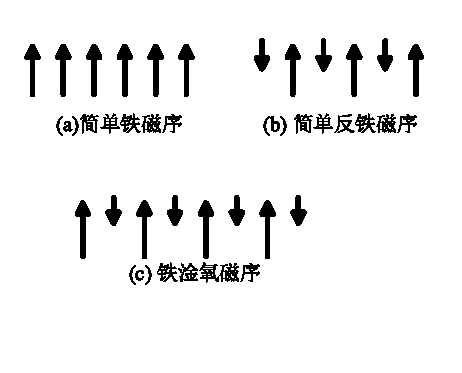
\includegraphics[width=6.5cm]{fig3-1.pdf}\\{\small 图 3.1\quad 自旋-自旋互作用系统的基态}
\end{minipage}
\end{center}

设铁磁体中某一个格点上的自旋 $\hat{\boldsymbol{S}}_l$ 因扰动偏离量子化轴方向，这时自旋间的交换作用使激发表现出如下特征：(i)$\hat{\boldsymbol{S}}_l$ 将带动近邻格点上自旋，而这些自旋又将使它们的近邻自旋取向改变，于是扰动以自旋集体运动的形式传播；(ii)近邻自旋对 $\hat{\boldsymbol{S}}_l$ 的作用要使它恢复原来取向以保持有序状态.这时在晶格中将形成离子自旋相对取向的振荡，图3.2是其经典图像.显然，由于各格点上进动自旋的方位角不同，磁激发具有类似波动的特性，这个波称为自旋波.

已经知道，通过弹性力耦合的晶格离子系统其低激发态是格波，而格波的量子称为声子.相似的，通过交换作用耦合的晶格自旋系统的低激发态以自旋波形式出现，自旋波的量子则称为磁振子.如果说声子是描述晶格离子间相对位移振荡的量子，那么磁振子就代表晶格自旋相对取向振荡的量子，它们都是互作用系统的集体激发.我们的任务是求铁磁体和反铁磁体中自旋波的频谱，涉及解自旋相互作用系统的本征态问题.为此，必须先考察自旋间相互作用的性质和哈密顿量的形式.

\begin{center}
\begin{minipage}{11cm}
\centering
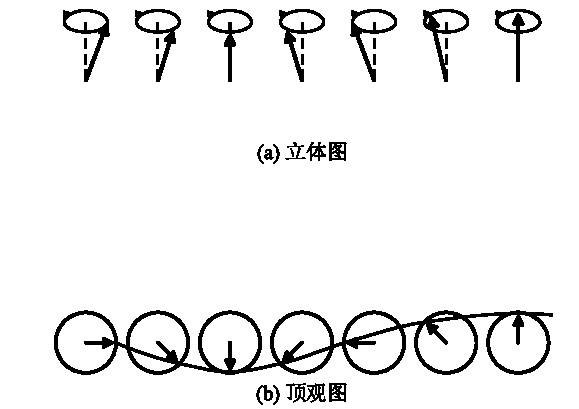
\includegraphics[width=11cm]{fig3-2.pdf}\\{\small 图 3.2\quad 自旋波的经典图像}
\end{minipage}
\end{center}

\section{海森伯模型及其严格推导}

\subsection*{1. 海森伯模型}

自旋-自旋相互作用系统的哈密顿量通常表示为
\begin{equation}
  H=-\sum_{l,l'}^{\prime}J_{ll'}\hat{\boldsymbol{S}}_l\cdot\hat{\boldsymbol{S}}_{l'}
\end{equation}
其中 $\hat{\boldsymbol{S}}_l$ 代表第 $l$ 个格点上磁性离子的矢量自旋算符，$\sum_{l,l'}^{\prime}$ 代表求和时不计 $l=l'$ 项，$J_{ll'}$ 是 $l$ 与 $l'$ 二格点离子上电子间的交换积分.
\begin{equation}
  J_{ll'}=J\left(\left|\boldsymbol{l}-\boldsymbol{l}'\right|\right)
\end{equation}
这里为简化记号令 $\boldsymbol{l}=\boldsymbol{R}_l$.式(3.2.1)与(3.2.2)就是海森伯模型\textsuperscript{[1]}，它是建立在如下一套假定之上的：

设两格点离子上各有一个自旋未配对的 d 电子，则根据量子力学，d 电子间交换能
\begin{equation}
  E_{\mathrm{ex}}=\pm J_{12}=\pm\int\phi_1^{*}\left(\boldsymbol{r}_1\right)\phi_2^{*}\left(\boldsymbol{r}_2\right)
  V\left(\boldsymbol{r}_{12}\right)\phi_1\left(\boldsymbol{r}_2\right)\phi_2\left(\boldsymbol{r}_1\right)
  \mathrm{d}\boldsymbol{r}_1\mathrm{d}\boldsymbol{r}_2
\end{equation}
其中 $V\left(\boldsymbol{r}\right)$ 为二格点系统的库仑互作用势，式(3.2.3)中正号对应于两个 d 电子自旋取向相反（$\uparrow\downarrow$）的状态，而负号代表两个 d 电子自旋取向一致（$\uparrow\uparrow$）.上式也可以等效地写为
\begin{equation*}
  E_{\mathrm{ex}}=\left\{\begin{array}{ll}
    +J_{12} & \mathcal{s}=0\\
    \left(\ \uparrow\downarrow\ ,\ \text{单重态}\right) & \\
    -J_{12} & \mathcal{s}=1\\
    \left(\ \uparrow\uparrow\ ,\ \text{三重态}\right) &
  \end{array}\right.
\end{equation*}
这里 $\mathcal{s}$ 为两格点间的组合自旋量子数，它是系统满足全同粒子不可区别性原理的直接结果.如用电子自旋算符描述，可求得两个电子系统的交换作用.由于
\begin{equation*}
  -\frac{1}{2}\left(1+4\hat{\mathcal{s}}_1\cdot\hat{\mathcal{s}}_2\right)
  =-\frac{1}{2}-\left(\hat{\boldsymbol{S}}^2-\hat{\mathcal{s}}_1^2-\hat{\mathcal{s}}_2^2\right)=\pm 1
\end{equation*}
其中 $+1$ 和 $-1$ 分别对应于总自旋算符 $\hat{\boldsymbol{S}}=\hat{\mathcal{s}}_1+\hat{\mathcal{s}}_2$ 的本征值取 $\mathcal{s}=0$ 或 $\mathcal{s}=1$，且有算符恒等式
\begin{equation*}
  \hat{\boldsymbol{S}}^2=\mathcal{s}\left(\mathcal{s}+1\right),\qquad
  \hat{\mathcal{s}}_1^2=\hat{\mathcal{s}}_2^2=\frac{1}{2}\left(\frac{1}{2}+1\right)=\frac{3}{4}
\end{equation*}
因此式(3.2.3)所对应的算符表示为
\begin{equation}
  H_{\mathrm{ex}}=-\frac{1}{2}J_{12}\left(1+4\hat{\mathcal{s}}_1\cdot\hat{\mathcal{s}}_2\right)
\end{equation}
略去常数项 $-\frac{1}{2}J_{12}$，求得两格点离子间的交换作用哈密顿量
\begin{equation}
  H_{12}=-2J_{12}\hat{\mathcal{s}}_1\cdot\hat{\mathcal{s}}_2
\end{equation}
尽管这里 $H_{12}$ 已表示成电子自旋矩间直接互作用的形式，但它来源于库仑势的交换作用项，互作用实为静电性的，不能理解为电子磁矩之间的直接磁作用.

将上式推广，应用到自旋大于 1/2 情况.这时每个离子上的自旋未配对 d 电子数大于 1，两格点间交换作用近似为
\begin{equation}
  H_{12}=-2J_{12}\sum_{i,j}\hat{\mathcal{s}}_{1i}\cdot\hat{\mathcal{s}}_{2j}
  =-2J_{12}\sum_i\hat{\mathcal{s}}_{1i}\cdot\sum_j\hat{\mathcal{s}}_{2j}
  =-2J_{12}\hat{\boldsymbol{S}}_1\cdot\hat{\boldsymbol{S}}_2
\end{equation}
其中 $\hat{\boldsymbol{S}}_1=\sum_i\hat{\mathcal{s}}_{1i}$，$\hat{\boldsymbol{S}}_2=\sum_j\hat{\mathcal{s}}_{2j}$ 分别为两格点上离子的总自旋算符.这里还作了两个假定：(i)同一格点的离子上的电子间交换作用可以忽略不计，(ii)两格点间所有电子具有相同的交换积分.

再进一步，计入所有格点间的交换作用推广到整个固体，就得到海森伯哈密顿量式(3.2.1).注意，当式(3.2.6)对 $l$、$l'$ 格点求和时应乘 1/2 因子以免计算重复.

在应用海森伯模型时，常采用更为简化的哈密顿量.考虑到交换积分的大小与格点间电子云的重叠程度有关，交换作用是短程作用，可以只计算近邻格点间的作用.若再假定 $J_{l,l+\delta}$ 为各向同性的常数 $J$，则海森伯模型表示为
\begin{equation}
  H=-J\sum_{l,\delta}\hat{\boldsymbol{S}}_l\cdot\hat{\boldsymbol{S}}_{l+\delta}
\end{equation}
$\delta$ 代表近邻格点间位置矢差.当 $J>0$ 时，式(3.2.7)的基态为铁磁序，当 $J<0$ 时可用于描述反铁磁性，当 $J<0$、并且近邻格点为不同磁离子（$S$ 不同）时，则描述亚铁磁性，即铁淦氧磁序.

\subsection*{2. 海森伯哈密顿量的推导}

在(1)中只介绍了海森伯引入交换作用的思路，而不是理论推导.狄拉克\textsuperscript{[2]}首先从多电子相互作用的哈密顿量出发导出了海森伯模型，其理论适用于磁性绝缘体，即晶体的电子处于局域化状态时式(3.2.1)可严格导出，下面仅介绍 $S=\frac{1}{2}$ 情况的推导.

设晶体中有 $N$ 个格点，每个格点上的离子只有一个未配对的局域态 d 电子.当研究 $N$ 个局域电子系统的交换作用时，我们应当采用瓦尼尔函数\footnote{关于瓦尼尔函数的详细讨论见第八章§8.}$a\left(\boldsymbol{r}-\boldsymbol{l}\right)$ 作基函数表示态矢量
$\Psi\left(\boldsymbol{r}\right)=\sum_{l,\sigma}C_{l\sigma}a\left(\boldsymbol{r}-\boldsymbol{l}\right)$.根据二次量子化的标准手续，用 $\Psi$ 对电子间库仑势 $\frac{e^2}{\left|\boldsymbol{r}-\boldsymbol{r}'\right|}$ 求平均，不难得到交换作用为
\begin{equation}
  H_{\mathrm{ex}}=-\frac{1}{2}\sum_{l,l'}^{\prime}\sum_{\sigma,\sigma'}J_{ll'}
  C_{l\sigma}^{+}C_{l\sigma'}C_{l'\sigma'}^{+}C_{l'\sigma}
\end{equation}
其中二体库仑积分
\begin{equation}
  J_{ll'}=e^2\int\frac{a^{*}\left(\boldsymbol{r}-\boldsymbol{l}\right)\,a\left(\boldsymbol{r}-\boldsymbol{l}'\right)\,
  a^{*}\left(\boldsymbol{r}'-\boldsymbol{l}'\right)\,a\left(\boldsymbol{r}'-\boldsymbol{l}\right)}
  {\left|\boldsymbol{r}-\boldsymbol{r}'\right|}\,\mathrm{d}^3r\,\mathrm{d}^3r'
\end{equation}
假如系统是绝缘体，则格点间无电子转移，即使跳跃电导也认为其概率很小可以忽略，这时每格点上只可能有一个未配对的 d 电子，它的自旋取向为朝上或朝下，但不存在空态和电子对态.换句话说，对于绝缘体应有 d 电子的单占据条件，它在数学上表示为下列算符形式，即
\begin{equation}
  C_{l\uparrow}^{+}C_{l\uparrow}+C_{l\downarrow}^{+}C_{l\downarrow}=1
\end{equation}
由式(3.2.10)不难求得泡利自旋算符
\begin{equation}
  \hat{\sigma}^{z}=\begin{pmatrix}1&0\\0&-1\end{pmatrix},\quad
  \hat{\sigma}^{+}=\begin{pmatrix}0&2\\0&0\end{pmatrix},\quad
  \hat{\sigma}^{-}=\begin{pmatrix}0&0\\2&0\end{pmatrix}
\end{equation}
和电子的产生及消灭算符之间有重要关系：
\begin{equation}
  \left.\begin{aligned}
    \hat{\sigma}^{z}&=C_{l\uparrow}^{+}C_{l\uparrow}-C_{l\downarrow}^{+}C_{l\downarrow}\\
    \hat{\sigma}_l^{+}&=2C_{l\uparrow}^{+}C_{l\downarrow}\\
    \hat{\sigma}_l^{-}&=2C_{l\downarrow}^{+}C_{l\uparrow}
  \end{aligned}\right\}
\end{equation}
其证明如下：

可以令
\begin{equation}
  C_{\uparrow}^{+}C_{\uparrow}\equiv\begin{pmatrix}1&0\\0&0\end{pmatrix}
\end{equation}
此矩阵作用于自旋朝上的单占据态 $\begin{pmatrix}1\\0\end{pmatrix}$ 得本征值 1，而作用于自旋朝下的单占据态
$\begin{pmatrix}0\\1\end{pmatrix}$ 其本征值为 0.这说明 $\begin{pmatrix}1&0\\0&0\end{pmatrix}$ 代表自旋朝上的占据数算符，与
$C_{\uparrow}^{+}C_{\uparrow}$ 的作用相同.因此，式(3.2.13)合理.将式(3.2.13)代入式(3.2.10)，又得到
\begin{equation}
  C_{\downarrow}^{+}C_{\downarrow}=\begin{pmatrix}0&0\\0&1\end{pmatrix}
\end{equation}
由于算符 $C_{\uparrow}^{+}C_{\downarrow}$ 使格点自旋从朝下态变为朝上态，故其作用应与
$\begin{pmatrix}0&1\\0&0\end{pmatrix}$ 相同.类似的，算符 $C_{\downarrow}^{+}C_{\uparrow}$ 应与
$\begin{pmatrix}0&0\\1&0\end{pmatrix}$ 作用相同.因此，还有下列对应关系：
\begin{equation}
  C_{\uparrow}^{+}C_{\downarrow}=\begin{pmatrix}0&1\\0&0\end{pmatrix},\quad
  C_{\downarrow}^{+}C_{\uparrow}=\begin{pmatrix}0&0\\1&0\end{pmatrix}
\end{equation}
利用式(3.2.13)—(3.2.15)，即可求出关系式(3.2.12)，或者换一个书写形式
\begin{equation}
  \left.\begin{aligned}
    C_{l\uparrow}^{+}C_{l\uparrow}&=\frac{1}{2}\left(1+\hat{\sigma}_l^{z}\right),&
    C_{l\downarrow}^{+}C_{l\downarrow}&=\frac{1}{2}\left(1-\hat{\sigma}_l^{z}\right)\\
    C_{l\uparrow}^{+}C_{l\downarrow}&=\frac{1}{2}\hat{\sigma}_l^{+},&
    C_{l\downarrow}^{+}C_{l\uparrow}&=\frac{1}{2}\hat{\sigma}_l^{-}
  \end{aligned}\right\}
\end{equation}
具体写出式(3.2.8)中的自旋求和
\begin{equation}
\begin{aligned}
  H_{\mathrm{ex}}=-\frac{1}{2}\sum_{l,l'}^{\prime}J_{ll'}\bigl\{&C_{l\uparrow}^{+}C_{l\uparrow}C_{l'\uparrow}^{+}C_{l'\uparrow}
  +C_{l\downarrow}^{+}C_{l\downarrow}C_{l'\downarrow}^{+}C_{l'\downarrow}\\
  &+C_{l\uparrow}^{+}C_{l\downarrow}C_{l'\downarrow}^{+}C_{l'\uparrow}
  +C_{l\downarrow}^{+}C_{l\uparrow}C_{l'\uparrow}^{+}C_{l'\downarrow}\bigr\}
\end{aligned}
\end{equation}
再将式(3.2.16)代入上式
\begin{equation}
\begin{aligned}
  H_{\mathrm{ex}}&=-\frac{1}{2}\sum_{l,l'}^{\prime}J_{ll'}\biggl\{\frac{1}{4}\left(1+\hat{\sigma}_l^{z}\right)\left(1+\hat{\sigma}_{l'}^{z}\right)
  +\frac{1}{4}\left(1-\hat{\sigma}_l^{z}\right)\left(1-\hat{\sigma}_{l'}^{z}\right)
  +\frac{1}{4}\hat{\sigma}_l^{+}\hat{\sigma}_{l'}^{-}+\frac{1}{4}\hat{\sigma}_l^{-}\hat{\sigma}_{l'}^{+}\biggr\}\\
  &=-\frac{1}{4}\sum_{l,l'}^{\prime}J_{ll'}\biggl\{\hat{\sigma}_l^{z}\hat{\sigma}_{l'}^{z}
  +\frac{1}{2}\left(\hat{\sigma}_l^{+}\hat{\sigma}_{l'}^{-}+\hat{\sigma}_l^{-}\hat{\sigma}_{l'}^{+}\right)+1\biggr\}\\
  &=-\frac{1}{4}\sum_{l,l'}^{\prime}J_{ll'}\left(\hat{\boldsymbol{\sigma}}_l\cdot\hat{\boldsymbol{\sigma}}_{l'}+1\right)
\end{aligned}
\end{equation}
略去常数项，并注意到当 $S=\frac{1}{2}$ 时 $\hat{\boldsymbol{S}}_l=\frac{1}{2}\hat{\boldsymbol{\sigma}}_l$，就导出了海森伯哈密顿式(3.2.1).在狄拉克理论基础上，安德逊(P.W.Anderson)\textsuperscript{[3]}进一步证明了海森伯模型也适用于 $S>\frac{1}{2}$ 情况.

\section{铁磁自旋波理论\textsuperscript{[4]}}

对于铁磁体，交换积分 $J>0$，设有 $N$ 个自旋为 $S$ 的磁离子排成晶格.现在的问题是求海森伯哈密顿量[式(3.2.7)]在 $J>0$ 时的平均值.尽管在一般情况下三维海森伯模型的严格解至今尚未找到.但是对于铁磁体的低激发态，可以通过变换使 $H$ 近似对角化，求得低温自旋波解.

\subsection*{1. 铁磁体的基态}

哈密顿量 $H$ 中所含矢量算符 $\hat{\boldsymbol{S}}_l=\left(\hat{S}_l^{x},\hat{S}_l^{y},\hat{S}_l^{z}\right)$ 的分量之间有对易关系
\begin{equation}
  \left[\hat{S}_l^{x},\hat{S}_{l'}^{y}\right]=\mathrm{i}\hat{S}_l^{z}\delta_{ll'}\qquad
  \left(x,y,z\ \text{循环}\right)
\end{equation}
为简单起见，这里和以后都以 $\hbar=1$.由于有算符等式
\begin{equation}
  \hat{\boldsymbol{S}}_l^{2}=\hat{\boldsymbol{S}}_l\cdot\hat{\boldsymbol{S}}_l=S\left(S+1\right)
\end{equation}
因此 $\hat{\boldsymbol{S}}_l$ 的 3 个分量不独立.在讨论自旋互作用系统特性时，常采用
$\hat{S}_l^{+}=\hat{S}_l^{x}+\mathrm{i}\hat{S}_l^{y}$ 与 $\hat{S}_l^{-}=\hat{S}_l^{x}-\mathrm{i}\hat{S}_l^{y}$ 作为独立变量，它们满足对易式
\begin{equation}
  \left.\begin{aligned}
    \left[\hat{S}_l^{\pm},\hat{S}_{l'}^{z}\right]&=\mp\hat{S}_l^{\pm}\delta_{ll'}\\
    \left[\hat{S}_l^{+},\hat{S}_{l'}^{-}\right]&=2\hat{S}_l^{z}\delta_{ll'}
  \end{aligned}\right\}
\end{equation}
设 $z$ 为量子化轴方向（或加一弱磁场使之稳定），则某一格点上的自旋态可用离子自旋 $S$ 与算符
$\hat{S}_l^{z}$ 的本征值 $m$ 标记为 $|S,\ m\rangle$，根据量子力学可知
\begin{equation}
  \left.\begin{aligned}
    \hat{S}_l^{+}|S,\ m\rangle&=\left[(S-m)(S+m+1)\right]^{\frac{1}{2}}|S,\ m+1\rangle\\
    \hat{S}_l^{-}|S,\ m\rangle&=\left[(S+m)(S-m+1)\right]^{\frac{1}{2}}|S,\ m-1\rangle
  \end{aligned}\right\}
\end{equation}
$\hat{S}_l^{\pm}$ 的作用分别为使 $l$ 格点上自旋沿 $z$ 轴的投影 $m$ 增加或减少一个量子数，这里的 $m$ 取
$0,\pm1,\pm2,\cdots\pm S$ 等 $\left(2S+1\right)$ 个数值.$\hat{S}_l^{\pm}$ 又称为自旋上升及下降算符.

若用 $\hat{S}_l^{z}$ 和 $\hat{S}_l^{\pm}$ 表示哈密顿量
\begin{equation}
  H=-J\sum_{l,\delta}^{\prime}\biggl\{\hat{S}_l^{z}\hat{S}_{l+\delta}^{z}
  +\frac{1}{2}\left(\hat{S}_l^{+}\hat{S}_{l+\delta}^{-}+\hat{S}_l^{-}\hat{S}_{l+\delta}^{+}\right)\biggr\}
\end{equation}
则可严格证明铁磁体的基态为
\begin{equation}
  |0\rangle\equiv|S\rangle_1|S\rangle_2\cdots|S\rangle_l\cdots|S\rangle_N
\end{equation}
其中 $|S\rangle_l$ 是 $|S,\ m=S\rangle_l$ 的缩写，这时每个格点上的自旋取向一致，它们都沿量子化轴方向.当 $H$
作用于态 $|0\rangle$ 时只有第一项 $\hat{S}_l^{z}\hat{S}_{l+\delta}^{z}$ 不为零，$H$ 中其它两项均无贡献.这是因为在
$|S\rangle_l$ 中 $m$ 已取最大值 $S$ 不能再上升，算符 $\hat{S}_l^{+}$ 作用的结果必为零
\begin{equation}
  \hat{S}_l^{+}|0\rangle=0
\end{equation}
又由于 $\sum_{\delta}^{\prime}$ 代表求和时 $\delta\neq0$，故无论 $\hat{S}_l^{+}$ 在 $\hat{S}_{l+\delta}^{-}$ 之前或其后，作用结果都一样，因此
\begin{equation}
  H|0\rangle=-J\biggl(\sum_{l,\delta}^{\prime}\hat{S}_l^{z}\hat{S}_{l+\delta}^{z}\biggr)|0\rangle=-JNZS^2|0\rangle
\end{equation}
其中利用了本征方程 $\hat{S}_l^{z}|S\rangle_l=S|S\rangle_l$，$Z$ 为晶格的配位数.由式(3.3.8)可知，状态
$|0\rangle$ 的本征值为
\begin{equation}
  E_0=-JNZS^2
\end{equation}
这里 $NZS^2$ 因子来源于态 $|0\rangle$ 中所有格点的 $\hat{S}_l^{z}$ 均取最大本征值 $m=S$.对于与
$|0\rangle$ 不同的其它自旋组态，至少应有一个格点的 $m<S$，则必然得到小于 $NZS^2$ 的结果.因此，$E_0$ 是
$H$ 的最低能量本征值，而 $|0\rangle$ 为 $H$ 的严格基态.

\subsection*{2. 霍斯坦因－普里马可夫变换}

现在讨论自旋系统的低激发态，设格点 $l$ 上自旋有偏转，例如从 $S$ 变为 $(S-1)$，如图3.3(a)所示.这个状态可表示为
\begin{equation*}
  |(S-1)_l\rangle\equiv|S\rangle_1\cdots|S\rangle_{l-1}|S-1\rangle_l|S\rangle_{l+1}\cdots|S\rangle_N
\end{equation*}

\begin{center}
\begin{minipage}{7cm}
\centering
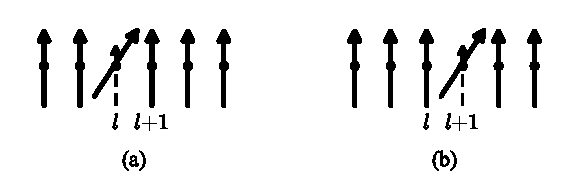
\includegraphics[width=7cm]{fig3-3.pdf}\\{\small 图 3.3}
\end{minipage}
\end{center}

哈密顿量 $H$ 中 $\hat{S}_l^{+}\hat{S}_{l+1}^{-}$ 项的作用使 $l$ 格点上偏转消失，而在 $(l+1)$
格点上产生新偏转[参看图3.3(b)]，状态 $|(S-1)_l\rangle$ 变为
\begin{equation*}
  |(S-1)_{l+1}\rangle=|S\rangle_1\cdots|S\rangle_l|S-1\rangle_{l+1}|S\rangle_{l+2}\cdots|S\rangle_N
\end{equation*}
偏转不再固定于 $l$ 格点上，它将在晶格中传播.这说明格点间的交换作用使得单个自旋偏转以集体激发的形式表现，与点阵位移在晶格中的传播相似.因此，在低激发态中少数自旋相对于量子化轴的偏离将因相互作用而被
$N$ 个自旋所平分.这时，每个自旋的平均偏离必然很小.

为了在数学上表示它们的相似性，也为了使 $H$ 对角化方便，我们引入量
\begin{equation}
  n\equiv S-m\qquad\left(m=0,\pm1,\cdots,\pm S\right)
\end{equation}
$n$ 代表自旋在量子化轴方向投影的偏离量，称为自旋偏离量子数.$n$ 取下列正整数：
\begin{equation}
  n=0,\ 1,\ 2,\ \cdots 2S\qquad\left(n\leqslant2S\right)
\end{equation}
与声子数相似.若用 $n$ 标记自旋态，则式(3.3.4)变换为
\begin{equation}
  \left.\begin{aligned}
    \hat{S}^{+}|n\rangle&=\sqrt{2S-(n-1)}\sqrt{n}\,|n-1\rangle\\
    \hat{S}^{-}|n\rangle&=\sqrt{2S-n}\sqrt{n+1}\,|n+1\rangle
  \end{aligned}\right\}
\end{equation}
显然，$\hat{S}^{+}$ 的作用使偏离趋于消灭，$\hat{S}^{-}$ 的作用为产生偏离.可以按常规引入对应于 $n$ 的产生和消灭算符
\begin{equation}
  a|n\rangle=\sqrt{n}\,|n-1\rangle,\qquad a^{+}|n\rangle=\sqrt{n+1}\,|n+1\rangle
\end{equation}
这时量子数 $n$ 的算符应为 $a^{+}a$，并且
\begin{equation}
  a^{+}a|n\rangle=n|n\rangle
\end{equation}
根据式(3.3.10)、(3.3.12)和(3.3.14)，容易找了下列算符变换关系：
\begin{equation}
  \left.\begin{aligned}
    \hat{S}^{+}&=\left(\sqrt{2S-a^{+}a}\right)a\\
    \hat{S}^{-}&=a^{+}\left(\sqrt{2S-a^{+}a}\right)\\
    \hat{S}^{z}&=\left(S-a^{+}a\right)
  \end{aligned}\right\}
\end{equation}
其中算符 $a$、$a^{+}$ 的对易式为
\begin{equation}
  \left[a,a^{+}\right]=1,\qquad\left[a,a\right]=\left[a^{+},a^{+}\right]=0
\end{equation}
下面将证明式(3.3.16)与自旋算符的对易式(3.3.3)是等价的.我们可以认为 $a^{+}$ 与 $a$
是玻色子的产生与消灭算符，唯一的差别只是这里的 $n$ 有限制，它不能超过 $2S$.

现在，由 $a$、$a^{+}$ 的对易式导出 $\hat{S}^{+}$、$\hat{S}^{-}$ 的对易式.
\begin{equation*}
\begin{aligned}
  \left[\hat{S}^{+},\hat{S}^{-}\right]&=\left(\sqrt{2S-a^{+}a}\right)aa^{+}\left(\sqrt{2S-a^{+}a}\right)
  -a^{+}\left(2S-a^{+}a\right)a\\
  &=\left(a^{+}a+1\right)\left(2S-a^{+}a\right)-a^{+}a\left(2S-a^{+}a\right)-a^{+}a\\
  &=2\left(S-a^{+}a\right)\\
  &=2\hat{S}^{z}
\end{aligned}
\end{equation*}
其中利用了 $\left[a^{+}a,a^{+}a\right]=0$ 和 $\left[a^{+}a,a\right]=-a$.

式(3.3.15)称为霍斯坦因－普里马可夫(Holstein-Primakoff)\textsuperscript{[5]}
变换，以后简称 HP 变换.将 HP 变换代入式(3.3.5)，得到海森伯哈密顿的二次量子化表示式
\begin{equation}
\begin{aligned}
  H=-J\sum_{l,\delta}^{\prime}\bigl\{&\left(S-a_l^{+}a_l\right)\left(S-a_{l+\delta}^{+}a_{l+\delta}\right)\\
  &+\frac{1}{2}\sqrt{2S-a_l^{+}a_l}\,a_l a_{l+\delta}^{+}\sqrt{2S-a_{l+\delta}^{+}a_{l+\delta}}\\
  &\left.+\frac{1}{2}a_l^{+}\sqrt{2S-a_l^{+}a_l}\sqrt{2S-a_{l+\delta}^{+}a_{l+\delta}}\,a_{l+\delta}\right\}
\end{aligned}
\end{equation}
算符的对易式可由式(3.3.16)推广得到
\begin{equation}
  \left[a_l,a_{l'}^{+}\right]=\delta_{l,l'},\qquad
  \left[a_l,a_{l'}\right]=\left[a_l^{+},a_{l'}^{+}\right]=0
\end{equation}
由于式(3.3.17)中含有偏离量子数 $n$ 所对应算符 $a^{+}a$ 的根号项，不仅使 $H$
的表示式变得十分复杂，而且对于激发态 $\left(n>0\right)$ 实际上无法求出 $H$ 的严格本征解，只能找近似解.所幸在低激发态每个自旋的平均偏离很小，这时可以将根号展开，并求得良好的低温近似解.

\subsection*{3. 低激发态——自旋波}

尽管式(3.3.17)比较复杂，但由于它用玻色粒子算符表示哈密顿量，将便于作低温展开使 $H$ 近似为可对角化的形式.

考虑与铁磁基态偏离不大的低激发态（即低温区），这时晶体中只有少数自旋发生了偏转，平均值
$\langle a_l^{+}a_l\rangle$ 应比 $2S$ 小得多，作为低阶近似可用 $\sqrt{2S}$
代替式(3.3.17)中的根号，再略去算符的四次方项，可将 $H$ 近似写为二次型
\begin{equation}
  H_0=-NZJS^2+2ZJS\sum_l a_l^{+}a_l
  -JS\sum_{l,\delta}^{\prime}\left(a_l a_{l+\delta}^{+}+a_l^{+}a_{l+\delta}\right)
\end{equation}
上式中第一项为基态能 $E_0$，第二项代表格点 $l$ 上的自旋偏离能，最后两项为不同格点间的耦合，它与简谐近似由位移表示的二次型哈密顿量相似.由于系统具有平移对称性，自旋的上升与下降算符
$\hat{S}_l^{\pm}$ 将与位移 $\boldsymbol{u}_l$ 相似，也可以用简正模
$N^{-\frac{1}{2}}\mathrm{e}^{-\mathrm{i}\boldsymbol{k}\cdot\boldsymbol{l}}$ 作展开表示 $\hat{S}_l^{\pm}$.再考虑到在低激态有近似关系
$\hat{S}_l^{+}=a_l\sqrt{2S}$ 及 $\hat{S}_l^{-}=a_l^{+}\sqrt{2S}$，可以设下列展开式：
\begin{equation}
  \left.\begin{aligned}
    a_l&=N^{-\frac{1}{2}}\sum_k\mathrm{e}^{\mathrm{i}\boldsymbol{k}\cdot\boldsymbol{l}}b_k\\
    a_l^{+}&=N^{-\frac{1}{2}}\sum_k\mathrm{e}^{-\mathrm{i}\boldsymbol{k}\cdot\boldsymbol{l}}b_k^{+}
  \end{aligned}\right\}
\end{equation}
这种类似于声子问题中引入简正坐标的办法，相当于对每个格点上的算符 $a_l$ 与 $a_l^{+}$
作点阵傅里叶变换.变换所引进的新算符由逆变换给出
\begin{equation}
  \left.\begin{aligned}
    b_k&=N^{-\frac{1}{2}}\sum_l\mathrm{e}^{-\mathrm{i}\boldsymbol{k}\cdot\boldsymbol{l}}a_l\\
    b_k^{+}&=N^{-\frac{1}{2}}\sum_l\mathrm{e}^{\mathrm{i}\boldsymbol{k}\cdot\boldsymbol{l}}a_l^{+}
  \end{aligned}\right\}
\end{equation}
显然，$b_k$ 与 $b_k^{+}$ 已不再是作用于某一格点上的算符，而是作用于所有格点的自旋波算符，代表自旋系统的集体坐标.新算符
$b_k$ 与 $b_k^{+}$ 同样满足玻色对易律
\begin{equation}
  \left.\begin{aligned}
    \left[b_k,b_{k'}^{+}\right]&=\delta_{kk'}\\
    \left[b_k,b_{k'}\right]&=\left[b_k^{+},b_{k'}^{+}\right]=0
  \end{aligned}\right\}
\end{equation}
将式(3.3.20)代入式(3.3.19)，再利用
$N^{-1}\sum_l\mathrm{e}^{\mathrm{i}\left(\boldsymbol{k}-\boldsymbol{k}'\right)\cdot\boldsymbol{l}}=\delta_{kk'}$，求得对角化的哈密顿量
\begin{equation}
\begin{aligned}
  H_0&=E_0+2ZJS\sum_k b_k^{+}b_k-ZJS\sum_k\gamma_k\left(b_kb_k^{+}+b_k^{+}b_k\right)\\
  &=E_0+\sum_k\hbar\omega_k b_k^{+}b_k
\end{aligned}
\end{equation}
$\omega_k$ 是自旋波频率，$\hbar\omega_k$ 代表自旋波的量子，简称为磁振子
\begin{equation}
  \hbar\omega_k=2ZJS\left(1-\gamma_k\right)
\end{equation}
其中定义了自旋波的结构因子
\begin{equation}
  \gamma_k=Z^{-1}\sum_\delta\mathrm{e}^{\mathrm{i}\boldsymbol{k}\cdot\boldsymbol{\delta}}=\gamma_{-k}
\end{equation}
$\gamma_k=\gamma_{-k}$ 是由于晶格有反演对称性，此外还有
\begin{equation}
  \sum_k\gamma_k=\sum_{\delta\neq0}\sum_k\frac{1}{Z}\mathrm{e}^{\mathrm{i}\boldsymbol{k}\cdot\boldsymbol{\delta}}=0
\end{equation}
不同结构晶体的 $\gamma_k$ 不同，因此求自旋波频率与波矢 $\boldsymbol{k}$
的关系时，应结合晶体对称性作计算.在低温情况下可利用长波条件
$\left|\boldsymbol{k}\cdot\boldsymbol{\delta}\right|<\!<1$ 展开 $\gamma_k$，求得 $\hbar\omega_k$ 的简单表示式
\begin{equation}
\begin{aligned}
  \hbar\omega_k&=2ZJS\left(1-\gamma_k\right)\\
  &\approx 2JS\biggl\{Z-\sum_\delta\biggl[1-\frac{1}{2}\left(\boldsymbol{k}\cdot\boldsymbol{\delta}\right)^2\biggr]\biggr\}\\
  &=JS\sum_\delta\left(\boldsymbol{k}\cdot\boldsymbol{\delta}\right)^2
\end{aligned}
\end{equation}
立方系的 3 种晶格（sc、bcc 和 fcc）有相同的长波色散关系
\begin{equation}
  \hbar\omega_k=2JSa^2k^2
\end{equation}
因为
$\sum_\delta\left(\boldsymbol{k}\cdot\boldsymbol{\delta}\right)^2
=\biggl\{\frac{1}{Z}\sum_\delta Z\delta^2\cos^2\theta\left(\boldsymbol{k},\boldsymbol{\delta}\right)\biggr\}k^2$，$\cos^2\theta\left(\boldsymbol{k},\boldsymbol{\delta}\right)$
的平均值为 $1/3$，$Z\delta^2$ 的平均值对 3 种晶格均为 $6a^2$，$a$ 是立方胞边长.

式(3.3.23)已将海森伯哈密顿变换为熟知的谐振子形式，其中 $b_k^{+}b_k=\hat{n}_k$
代表自旋波量子的数密度算符，其本征值即是在 $\boldsymbol{k}$
波矢自旋波上所激发自旋波量子的个数，而 $b_k^{+}$ 与 $b_k$
又称为自旋波量子的产生及消灭算符.与声子问题相似，用自旋波量子数表示的态向量
$|n_1,\cdots,n_N\rangle$ 是 $H_0$ 的本征向量，因此 $H_0$ 通常又称为自旋波近似的哈密顿量.

若展开式(3.3.17)中根号
\begin{equation}
  \sqrt{1-a^{+}a/2S}=1-\frac{1}{2}\left(\frac{a^{+}a}{2S}\right)+\frac{1}{8}\left(\frac{a^{+}a}{2S}\right)^2+\cdots
\end{equation}
计入算符的高阶项的影响，可得
\begin{equation}
  H=H_0+H_1+\cdots
\end{equation}
其中
\begin{equation}
  H_1=\frac{ZJ}{2N}\sum_{k,k',q}\left(\gamma_{k-q}+\gamma_{k'}-2\gamma_{k-q-k'}\right)
  b_{k-q}^{+}b_{k'+q}^{+}b_{k'}b_k
\end{equation}
代表自旋波之间的相互作用，它消灭 $\boldsymbol{k}$ 与 $\boldsymbol{k}'$ 量子并产生
$\boldsymbol{k}-\boldsymbol{q}$，$\boldsymbol{k}'+\boldsymbol{q}$ 量子，是典型的准粒子互作用项.

从式(3.3.19)不难看出，自旋波只是下列线性化运动方程的解
\begin{equation}
  \mathrm{i}\hbar\frac{\partial a_l}{\partial t}=\left[a_l,H_0\right]
  =2ZJSa_l-JS\sum_{\delta}^{\prime}\left(a_{l+\delta}+a_{l-\delta}\right)
\end{equation}
因为只需对上式作傅里叶变换，即可得到自旋波的算符方程
\begin{equation}
  \mathrm{i}\hbar\frac{\partial b_k}{\partial t}=2ZJS\left(1-\gamma_k\right)b_k=\hbar\omega_kb_k
\end{equation}
其中 $\hbar\omega_k$ 就是磁振子的能量，说明自旋波以 $\omega_k$
频率振荡.所以，前面求出的自旋波模式只是线性理论的结果，而磁振子可称为系统的线性元激发.如果进一步考虑自旋波之间的相互作用，我们将得到算符
$a_l$
的非线性方程.在一维情况下，这个非线性方程有孤子解，孤子代表系统的非线性元激发，我们将在本章§7中介绍.

自旋波之间的相互作用对于 $\omega_k$ 有重要的修正效应.若从 $H_0+H_1$ 出发，建立 $b_k$ 的运动方程
\begin{equation}
  \mathrm{i}\hbar\dot{b}_k=\left[b_k,H_0\right]+\left[b_k,H_1\right]
\end{equation}
再利用对易关系式(3.3.22)和 $H_0$ 及 $H_1$ 的表示式(3.3.23)和(3.3.31)，可算出
\begin{equation}
  \left[b_k,H_0\right]=2ZJS\left(1-\gamma_k\right)b_k
\end{equation}
\begin{equation}
\begin{aligned}
  \left[b_k,H_1\right]=\frac{ZJ}{2N}\sum_{k',q}\biggl\{&\left(\gamma_k+\gamma_{k'}-2\gamma_{k-k'}\right)
  b_{k'+q}^{+}b_{k+q}b_{k'}\\
  &+\left(\gamma_{k-q}+\gamma_{k'-q}-2\gamma_{k-k'}\right)b_{k'-q}^{+}b_{k-q}b_{k'}\biggr\}
\end{aligned}
\end{equation}
为了得到互作用项 $H_1$ 对于自旋波频谱的修正，对上式作线性化近似
\begin{equation}
  b_k^{+}b_{k_1}b_{k_2}\approx\left(\delta_{kk_1}b_{k_2}+\delta_{kk_2}b_{k_1}\right)\langle b_k^{+}b_k\rangle_T
\end{equation}
其中
\begin{equation}
  \langle b_k^{+}b_k\rangle_T=\left\{\mathrm{e}^{\hbar\omega_k/k_{\mathrm{B}}T}-1\right\}^{-1}
  =\langle\hat{n}_k\rangle_T
\end{equation}
再利用等式
\begin{equation*}
  \gamma_{k-k'}=\gamma_{k'-k}
\end{equation*}
和
\begin{equation}
  \sum_{k'}\gamma_{k-k'}\langle\hat{n}_{k'}\rangle_T=\gamma_k\sum_{k'}\gamma_{k'}\langle\hat{n}_{k'}\rangle_T
\end{equation}
经整理后得到下列线性方程
\begin{equation}
  \mathrm{i}\hbar\dot{b}_k=\hbar\omega_k\left(T\right)b_k
\end{equation}
求出修正后的自旋波量子与温度 $T$ 有关，其表示式为
\begin{equation}
  \hbar\omega_k\left(T\right)=2ZJS\left(1-\gamma_k\right)\left\{\frac{1-e\left(T\right)}{S}\right\}
\end{equation}
这里
\begin{equation}
  e\left(T\right)\equiv\frac{1}{N}\sum_{k'}\left(1-\gamma_{k'}\right)\langle\hat{n}_{k'}\rangle_T
\end{equation}
显然，相互作用对自旋波量子的修正归结为重正因子 $\left\{\frac{1-e\left(T\right)}{S}\right\}$
，这个因子随温度升高而减少，表明当温度升高时会发生自旋波频率的软化现象，从而导致失稳.具体计算
$\hbar\omega_k\left(T\right)$
时，应当联立式(3.3.38)、(3.3.41)和(3.3.42)自洽求解.图3.4
是铁磁绝缘材料 $\mathrm{EuO}$ 中 $\hbar\omega_k\left(T\right)$
的实验与理论比较\textsuperscript{[6]}，其中 $\square$、$\triangle$、$\circ$、$\bullet$
代表不同波矢自旋波量子的测量值，实线为上述理论的自洽解，显然两者符合较好.

\begin{center}
\begin{minipage}{8cm}
\centering
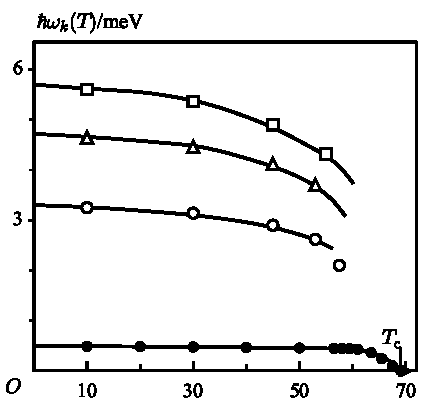
\includegraphics[width=8cm]{fig3-4.pdf}\\{\small
  图 3.4\quad $\mathrm{EuO}$ 的 $\hbar\omega_k(T)$ 曲线，$T_{\mathrm{c}}=69.1\ \mathrm{K}$\\
  $k=2\ \mathrm{nm}^{-1}(\bullet)$，$6\ \mathrm{nm}^{-1}(\circ)$，$8\ \mathrm{nm}^{-1}(\triangle)$，$10\ \mathrm{nm}^{-1}(\square)$}
\end{minipage}
\end{center}

\section{铁磁体的低温磁化强度}

由于自旋波算符满足玻色对易关系，因此温度为 $T$ 时 $\boldsymbol{k}$
自旋波所激发量子的平均数应按玻色分布决定，即
\begin{equation}
  \langle\hat{n}_k\rangle_T=\langle b_k^{+}b_k\rangle_T
  =\frac{1}{\mathrm{e}^{\hbar\omega_k/k_{\mathrm{B}}T}-1}
\end{equation}
低温时所有自旋波模的总元激发个数可利用式(3.3.28)写为
\begin{equation}
  \sum_k\langle\hat{n}_k\rangle_T=\frac{V}{8\pi^3}\int_{\Omega^{*}}
  \frac{\mathrm{d}^3k}{\exp\left[2SJa^2k^2/k_{\mathrm{B}}T\right]-1}
\end{equation}
设温度足够低，$2SJa^2k_{\mathrm{max}}^2>\!>k_{\mathrm{B}}T$，积分可以近似在全 $\boldsymbol{k}$ 空间进行，经整理后得
\begin{equation}
\begin{aligned}
  \frac{1}{N}\sum_k\langle\hat{n}_k\rangle_T
  &=\left(\frac{V}{2Na^3}\right)\cdot\left(\frac{k_{\mathrm{B}}T}{2JS}\right)^{3/2}
  \cdot\left(\frac{1}{2\pi^2}\int_0^{\infty}\frac{x^{\frac{1}{2}}\mathrm{d}x}{\mathrm{e}^{x}-1}\right)\\
  &=\left(\frac{V}{2Na^3}\right)\cdot\left(\frac{k_{\mathrm{B}}T}{2JS}\right)^{3/2}
  \cdot\frac{1}{2\pi^2}\Gamma\left(\frac{3}{2}\right)\zeta\left(\frac{3}{2}\right)\\
  &=\left(\frac{k_{\mathrm{B}}T}{2SJ}\right)^{3/2}\alpha
\end{aligned}
\end{equation}
其中 $x\equiv\left(2SJa^2k^2/k_{\mathrm{B}}T\right)$，$\Gamma\left(\frac{3}{2}\right)=\frac{1}{2}\sqrt{\pi}$
，而黎曼函数 $\zeta\left(\frac{3}{2}\right)=2.612$.
对于 sc、bcc 和 fcc 晶格 $\left(\frac{V}{2Na^3}\right)$ 分别为
$\frac{1}{2}$、$\frac{1}{4}$ 和 $\frac{1}{8}$，因此 $\alpha$ 分别等于
$\frac{0.117}{2}$(sc)、$\frac{0.117}{4}$(bcc) 和 $\frac{0.117}{8}$(fcc).
当取体积 $V=1$ 时，铁磁体的低温磁化强度为
\begin{equation}
\begin{aligned}
  M\left(T\right)&=g\mu_{\mathrm{B}}\sum_l\left(S-\langle a_l^{+}a_l\rangle_T\right)\\
  &=Ng\mu_{\mathrm{B}}S-g\mu_{\mathrm{B}}\sum_k\left(\langle b_k^{+}b_k\rangle_T\right)\\
  &=M\left(0\right)\left\{1-\frac{1}{NS}\sum_k\langle\hat{n}_k\rangle_T\right\}\\
  &=M\left(0\right)\left\{1-\frac{\alpha}{S}\left(\frac{k_{\mathrm{B}}T}{2SJ}\right)^{3/2}\right\}
\end{aligned}
\end{equation}
其中 $M\left(0\right)=Ng\mu_{\mathrm{B}}S$
代表零温饱和磁化.由于自旋波激发所引起磁化强度的减小为
\begin{equation}
\begin{aligned}
  \Delta M\left(T\right)&=M\left(0\right)-M\left(T\right)\\
  &=M\left(0\right)\frac{\alpha}{S}\left(\frac{k_{\mathrm{B}}T}{2SJ}\right)^{3/2}\sim T^{3/2}
\end{aligned}
\end{equation}
这个结果是布洛赫\textsuperscript{[7]}最早求得的，其形式与实验得到的相同，称为布洛赫 $T^{3/2}$ 定律.

众所周知，用平均场理论求出的低温磁化强度为
\begin{equation}
  M\left(T\right)=M\left(0\right)\left\{1-\frac{1}{S}\mathrm{e}^{-\frac{3T_{\mathrm{c}}}{\left(S+1\right)T}}\right\}
\end{equation}
其中 $T_{\mathrm{c}}$ 为铁磁体的居里温度，
\begin{equation}
  T_{\mathrm{c}}=\frac{2}{3}\frac{ZJ}{k_{\mathrm{B}}}S\left(S+1\right)
\end{equation}
显然，平均场的结果表明 $\Delta M\left(T\right)$
按指数衰数，显然与实验不符.现在分析低温下平均场理论失败的原因.平均场理论将 $l$
格点自旋受到其它格点上自旋的海森伯交换作用近似为
\begin{equation}
  \mathcal{H}_l\approx-2\hat{\boldsymbol{S}}_l\cdot\biggl\{\sum_{l'}J_{ll'}\langle\hat{\boldsymbol{S}}_{l'}\rangle\biggr\}
\end{equation}
这里将 $\hat{\boldsymbol{S}}_{l'}$ 算符用平均值代替，从而定义了一个有效磁场 $\boldsymbol{h}_{\mathrm{eff}}$
\begin{equation}
  g\mu_{\mathrm{B}}\boldsymbol{h}_{\mathrm{eff}}\equiv2\sum_{l'}J_{ll'}\langle\hat{\boldsymbol{S}}_{l'}\rangle
  \approx2ZJ\langle\hat{\boldsymbol{S}}\rangle
\end{equation}
其中 $Z$ 为配位数，$g$ 是朗德因子，$\mu_{\mathrm{B}}$
是玻尔磁子，并考虑到铁磁体各格点上是相同自旋的离子，可略去平均量 $\langle\hat{\boldsymbol{S}}_l\rangle$ 的
$l$ 脚标.由于磁化强度 $\boldsymbol{M}=Ng\mu_{\mathrm{B}}\langle\hat{\boldsymbol{S}}\rangle$，因此
$\boldsymbol{h}_{\mathrm{eff}}\sim\boldsymbol{M}$，它就是外斯分子场.
式(3.4.8)称为海森伯互作用的平均场近似，它使多自旋互作用问题简化为平均场中的单自旋运动.这时任一自旋的哈密顿量为
\begin{equation*}
  \mathcal{H}=-\lambda g\mu_{\mathrm{B}}\hat{S}^{z}M
  \left[\lambda=\frac{2ZJ}{N\left(g\mu_{\mathrm{B}}\right)^2}\right]
\end{equation*}
其本征值为
\begin{equation}
  E_m=-\lambda g\mu_{\mathrm{B}}m\,M\qquad\left(m=0,\pm1,\cdots,\pm S\right)
\end{equation}
磁化强度为
\begin{equation}
  M\left(T\right)=Ng\mu_{\mathrm{B}}\langle\hat{S}^{z}\rangle
  =Ng\mu_{\mathrm{B}}\frac{\displaystyle\sum_{m=-S}^{S}m\,\mathrm{e}^{-\beta E_m}}
  {\displaystyle\sum_{m=-S}^{S}\mathrm{e}^{-\beta E_m}}
  =M\left(0\right)B_s(x)\quad\left[\beta=\left(k_{\mathrm{B}}T\right)^{-1}\right]
\end{equation}
这里布里渊函数
\begin{equation}
\begin{aligned}
  B_s\left(x\right)&=\left(\frac{2S+1}{2S}\right)\coth\biggl\{\left(\frac{2S+1}{2S}\right)x\biggr\}
  -\frac{1}{2S}\coth\biggl\{\left(\frac{1}{2S}\right)x\biggr\}\\
  &\qquad\qquad\left(x=\lambda g\mu_{\mathrm{B}}\frac{SM}{k_{\mathrm{B}}T}\right)
\end{aligned}
\end{equation}
利用高温展开式
\begin{equation}
  B_s\left(x\right)\approx\frac{S+1}{S}\,\frac{x}{3}\qquad\left(x<\!<1\right)
\end{equation}
可确定居里温度 $T_{\mathrm{c}}$ 与交换积分 $J$
的关系，求得式(3.4.7).当 $T<\!<T_{\mathrm{c}}$ 时，利用低温展开式
\begin{equation}
  B_s\left(x\right)\approx1-\frac{1}{S}\mathrm{e}^{-\frac{x}{S}}\qquad
  \left(\mathrm{e}^{-\frac{x}{S}}<\!<1\right)
\end{equation}
可导出平均场的低温 $M(T)$ 公式(3.4.6).显然，平均场理论只考虑了自旋运动的单体效应，它不能反映低温区自旋系统的集体激发特征.集体激发是多体效应，涉及自旋关联，其具体表现为：当任一自旋受其它
$(N-1)$ 个自旋作用而改变取向时，其它自旋的取向也将同时变化，这是海森伯互作用
$\hat{\boldsymbol{S}}_l\cdot\hat{\boldsymbol{S}}_{l'}$
算符特性的表现，称为自旋间的动力学关联.平均场理论在低温区失效的原因就是由于忽略了动力学关联，而自旋波理论则考虑了这种关联，所以取得了成功.

此外，容易算出铁磁体中磁振子的低温比热容
\begin{equation}
  c_m=\nu Nk_{\mathrm{B}}\left(\frac{k_{\mathrm{B}}T}{2JS}\right)^{3/2}
\end{equation}
其中常数 $\nu$ 对于 sc、bcc 和 fcc 晶格分别为 0.113、0.113/2 和 0.113/4.

在结束本节之前，我们还将导出自旋波的经典图像，根据对角化的哈密顿量式(3.3.23)，易求出
$\boldsymbol{k}$ 模自旋波算符的含时解为
$b_k\left(t\right)=b_k\left(0\right)\mathrm{e}^{-\mathrm{i}\omega_kt}$
，代入式(3.3.20)可将每个格点的自旋偏离算符写成
\begin{equation}
  \left.\begin{aligned}
    a_l\left(t\right)&=N^{-\frac{1}{2}}\sum_kb_k\left(0\right)
    \mathrm{e}^{\mathrm{i}\left(\boldsymbol{k}\cdot\boldsymbol{l}-\omega_kt\right)}\\
    a_l^{+}\left(t\right)&=N^{-\frac{1}{2}}\sum_kb_k^{+}\left(0\right)
    \mathrm{e}^{-\mathrm{i}\left(\boldsymbol{k}\cdot\boldsymbol{l}-\omega_kt\right)}
  \end{aligned}\right\}
\end{equation}
再考虑到在低激发态可以将自旋的上升与下降算符分别用 $a_l\sqrt{2S}$ 与
$a_l^{+}\sqrt{2S}$ 近似表示，这时低激发态的自旋振荡解为
\begin{equation}
  \left.\begin{aligned}
    \hat{S}_l^{+}\left(t\right)&=\sqrt{\frac{2S}{N}}\sum_kb_k\left(0\right)
    \mathrm{e}^{\mathrm{i}\left(\boldsymbol{k}\cdot\boldsymbol{l}-\omega_kt\right)}\\
    \hat{S}_l^{-}\left(t\right)&=\sqrt{\frac{2S}{N}}\sum_kb_k^{+}\left(0\right)
    \mathrm{e}^{\mathrm{i}\left(\boldsymbol{k}\cdot\boldsymbol{l}-\omega_kt\right)}
  \end{aligned}\right\}
\end{equation}
对上式作经典近似，将算符 $b_k\left(0\right)$ 与 $b_k^{+}\left(0\right)$
取为实 c 数，相应的将上升、下降算符 $\hat{\boldsymbol{S}}_l^{\pm}$
看成是经典矢量 $\boldsymbol{S}_l$ 的横向分量 $S_l^{\pm}$，再利用
$S_l^{x}=\frac{1}{2}\left(S_l^{+}+S_l^{-}\right)$ 及
$S_l^{y}=\frac{1}{2\mathrm{i}}\left(S_l^{+}-S_l^{-}\right)$，求出
$\boldsymbol{k}$ 模自旋波的经典近似解
\begin{equation}
  \left.\begin{aligned}
    S_l^{x}\left(t\right)&\sim\cos\left(\boldsymbol{k}\cdot\boldsymbol{l}-\omega_kt\right)\\
    S_l^{y}\left(t\right)&\sim\sin\left(\boldsymbol{k}\cdot\boldsymbol{l}-\omega_kt\right)
  \end{aligned}\right\}
\end{equation}
显然，上式表明：任一格点上的自旋都可以看成是经典的矢量，它们在 $Oxy$
平面内作圆周运动，并且相邻格点之间有确定的相位差（由 $\boldsymbol{k}\cdot\boldsymbol{l}$
决定），正如图3.2(b)所示.这就是图3.2中自旋波经典图像的来源.

\section{反铁磁自旋波理论}

当海森伯哈密顿量中 $J<0$ 时，近邻格点上的自旋趋于反平行排列，这时往往可以把晶格分为两个子格，在每个子格中自旋平行排列与铁磁情况一样，但两个子格的自旋取向相反，因此总的自发磁化相互抵消，这就是反铁磁体的双子格模型.例如在反铁磁材料
$\mathrm{MnF}_2$、$\mathrm{FeF}_2$ 和 $\mathrm{CoF}_2$
中，磁离子（$\mathrm{Mn}^{2+}$、$\mathrm{Fe}^{2+}$ 和
$\mathrm{Co}^{2+}$）排成体心四方晶格，它们可划分为两个简单四方子格.

\subsection*{1. 双子格模型}

我们将从双子格模型出发，讨论海森伯哈密顿量的基态和激发态.设每个子格中自旋数为 $N$，总的磁离子数为
$2N$，并取体积 $V=1$.$H$ 用 $a$、$b$ 两子格的自旋符表示
\begin{equation}
\begin{aligned}
  H={}&\left|J\right|\sum_{i,\delta}\biggl\{\hat{S}_{ai}^{z}\hat{S}_{b,i+\delta}^{z}
  +\frac{1}{2}\left(\hat{S}_{ai}^{+}\hat{S}_{b,i+\delta}^{-}+\hat{S}_{ai}^{-}\hat{S}_{b,i+\delta}^{+}\right)\biggr\}\\
  &+\left|J\right|\sum_{j,\delta}\biggl\{\hat{S}_{bj}^{z}\hat{S}_{a,j+\delta}^{z}
  +\frac{1}{2}\left(\hat{S}_{bj}^{+}\hat{S}_{a,j+\delta}^{-}+\hat{S}_{bj}^{-}\hat{S}_{a,j+\delta}^{+}\right)\biggr\}
\end{aligned}
\end{equation}
其中 $\hat{\boldsymbol{S}}_{ai}$ 代表子格 $a$ 中 $i$
格点上自旋算符，$\hat{\boldsymbol{S}}_{bj}$ 为 $b$ 子格中 $j$
格点上自旋.假设子格 $a$ 的量子化轴沿 $(+z)$ 方向，$b$ 沿 $(-z)$
方向，我们将所有 $a$ 子格中自旋沿 $(+z)$ 向排列，$b$ 中沿 $(-z)$
向排列的状态[如图3.1(b)]称为出发状态 $|\mathrm{Origin}\rangle$，则存在着与式(3.3.7)相似的关系
\begin{equation}
  \hat{S}_{ai}^{+}|\mathrm{Origin}\rangle=\hat{S}_{bj}^{-}|\mathrm{Origin}\rangle=0
\end{equation}
它说明 $\hat{S}_{ai}^{+}$ 对应于子格 $a$ 中的消灭算符，$\hat{S}_{bj}^{-}$
对应于 $b$ 子格的消灭算符，由于 $a$
子格自旋朝上，可仿铁磁情况作霍斯坦因－普里马可夫变换引入子格 $a$ 的产生及消灭算符
\begin{equation}
  \left.\begin{aligned}
    \hat{S}_{ai}^{+}&=\left(\sqrt{2S-a_i^{+}a_i}\right)a_i\\
    \hat{S}_{ai}^{-}&=a_i^{+}\sqrt{2S-a_i^{+}a_i}\\
    \hat{S}_{ai}^{z}&=S-a_i^{+}a_i
  \end{aligned}\right\}
\end{equation}
对于 $b$ 子格 $\hat{\boldsymbol{S}}^{+}$ 与 $\hat{\boldsymbol{S}}^{-}$ 的作用将颠倒，应定义
\begin{equation}
  \left.\begin{aligned}
    \hat{S}_{bj}^{+}&=b_j^{+}\sqrt{2S-b_j^{+}b_j}\\
    \hat{S}_{bj}^{-}&=\left(\sqrt{2S-b_j^{+}b_j}\right)b_j\\
    \hat{S}_{bj}^{z}&=b_j^{+}b_j-S
  \end{aligned}\right\}
\end{equation}
由于 $b$
子格的自旋上升是相对于量子化轴 $(-z)$ 的偏离增大，因此 $\hat{\boldsymbol{S}}_b^{+}$
对应于产生算符 $b^{+}$，$b$ 子格中 $\hat{\boldsymbol{S}}_b^{z}$
的定义与 $a$
子格相差负号的原因也是类似的，它可以从对易关系证明
\begin{equation*}
\begin{aligned}
  \left[\hat{S}_{bj}^{+},\hat{S}_{bj}^{-}\right]&=b_j^{+}\sqrt{2S-b_j^{+}b_j}\sqrt{2S-b_j^{+}b_j}\,b_j
  -\left(\sqrt{2S-b_j^{+}b_j}\right)b_jb_j^{+}\left(\sqrt{2S-b_j^{+}b_j}\right)\\
  &=b_j^{+}b_j\left(2S-b_j^{+}b_j\right)+b_j^{+}b_j
  -b_j^{+}b_j\left(2S-b_j^{+}b_j\right)-\left(2S-b_j^{+}b_j\right)\\
  &=2\left(b_j^{+}b_j-S\right)
\end{aligned}
\end{equation*}
与 $\left[\hat{S}_{bj}^{+},\hat{S}_{bj}^{-}\right]=2\hat{S}_{bj}^{z}$
相比较，可得式(3.5.4)的第 3 个等式.

$a_i$、$b_j$ 都是玻色算符，它们满足对易关系
\begin{equation}
\begin{aligned}
  &\left[a_i,a_{i'}^{+}\right]=\delta_{ii'},\qquad
  \left[a_i,a_{i'}\right]=\left[a_i^{+},a_{i'}^{+}\right]=0\\
  &\left[b_j,b_{j'}^{+}\right]=\delta_{jj'},\qquad
  \left[b_j,b_{j'}\right]=\left[b_j^{+},b_{j'}^{+}\right]=0\\
  &\left[a_i,b_j\right]=\left[a_i^{+},b_j\right]=\left[a_i,b_j^{+}\right]=\left[a_i^{+},b_j^{+}\right]=0
\end{aligned}
\end{equation}
对于低激发态，可用下列近似：
\begin{equation}
\begin{aligned}
  &\hat{S}_{ai}^{+}=(2S)^{\frac{1}{2}}a_i,\qquad
  \hat{S}_{ai}^{-}=(2S)^{\frac{1}{2}}a_i^{+},\qquad
  \hat{S}_{ai}^{z}=S-a_i^{+}a_i\\
  &\hat{S}_{bj}^{+}=(2S)^{\frac{1}{2}}b_j^{+},\qquad
  \hat{S}_{bj}^{-}=(2S)^{\frac{1}{2}}b_j,\qquad
  \hat{S}_{bj}^{z}=b_j^{+}b_j-S
\end{aligned}
\end{equation}
代入式(3.5.1)，并略去 $\hat{\boldsymbol{S}}_a^{z}\hat{\boldsymbol{S}}_b^{z}$
中算符 $a$、$b$ 的四次项，求得低温近似的哈密顿量
\begin{equation}
\begin{aligned}
  H={}&-2NZS^2\left|J\right|+2ZS\left|J\right|\biggl(\sum_i a_i^{+}a_i+\sum_j b_j^{+}b_j\biggr)\\
  &+2\left|J\right|S\sum_{i,\delta}\left(a_ib_{i+\delta}+a_i^{+}b_{i+\delta}^{+}\right)
\end{aligned}
\end{equation}
其中 $N$ 为子格中自旋数.仿照铁磁情况作傅里叶变换，分别对各子格引入自旋波算符 $a_k$、$b_k$：
\begin{equation}
  \left.\begin{aligned}
    a_i&=N^{-\frac{1}{2}}\sum_k\mathrm{e}^{\mathrm{i}\boldsymbol{k}\cdot\boldsymbol{R}_i}a_k\,,&
    a_i^{+}&=N^{-\frac{1}{2}}\sum_k\mathrm{e}^{-\mathrm{i}\boldsymbol{k}\cdot\boldsymbol{R}_i}a_k^{+}\\
    b_j&=N^{-\frac{1}{2}}\sum_k\mathrm{e}^{-\mathrm{i}\boldsymbol{k}\cdot\boldsymbol{R}_j}b_k\,,&
    b_j^{+}&=N^{-\frac{1}{2}}\sum_k\mathrm{e}^{\mathrm{i}\boldsymbol{k}\cdot\boldsymbol{R}_j}b_k^{+}
  \end{aligned}\right\}
\end{equation}
$\boldsymbol{R}_i$、$\boldsymbol{R}_j$ 为子格 $a$、$b$
的矢量，变换后的算符 $a_k$、$b_k$ 分别满足玻色对易关系
\begin{equation}
  \left[a_k,a_{k'}^{+}\right]=\left[b_k,b_{k'}^{+}\right]=\delta_{kk'}
\end{equation}
其它的对易式均等于零，算符 $a_k$ 与 $b_k$ 之间也可对易：
\begin{equation}
  \left[a_k,b_{k'}\right]=\left[a_k,b_{k'}^{+}\right]=\left[a_k^{+},b_{k'}\right]=\left[a_k^{+},b_{k'}^{+}\right]=0
\end{equation}
用双子格自旋波算符表示的哈密顿量为
\begin{equation}
\begin{aligned}
  H={}&-2NZS^2\left|J\right|+2ZS\left|J\right|\sum_k\left(a_k^{+}a_k+b_k^{+}b_k\right)\\
  &+2ZS\left|J\right|\sum_k\gamma_k\left(a_k^{+}b_k^{+}+b_ka_k\right)
\end{aligned}
\end{equation}
上式中第一项是出发状态的能量，第二项代表各子格中自旋波，第三项为交叉项代表两子格自旋波的相互作用.
式(3.5.11)说明本征模式应当是两个子格自旋波的组合.我们必须进一步作变换，引入组合的自旋波算符，才能消除交叉项，使
$H$ 对角化.

\subsection*{2. 玻戈留玻夫正则变换}

如何组合两个子格中的自旋波算符？让我们先考察子格算符的运动方程
\begin{equation}
  \left.\begin{aligned}
    \mathrm{i}\hbar\dot{a}_k&=\left[a_k,H\right]=2ZS\left|J\right|\left(a_k+\gamma_kb_k^{+}\right)\\
    \mathrm{i}\hbar\dot{b}_k&=\left[b_k,H\right]=2ZS\left|J\right|\left(b_k+\gamma_ka_k^{+}\right)
  \end{aligned}\right\}
\end{equation}
上式说明，应当组合 $a_k$ 与 $b_k^{+}$ 以及 $b_k$ 与 $a_k^{+}$
构成两套新的自旋波算符 $\alpha_k$ 和 $\beta_k$
\begin{equation}
  \left.\begin{aligned}
    \alpha_k&=u_ka_k-v_kb_k^{+}\ ,&\quad \alpha_k^{+}&=u_ka_k^{+}-v_kb_k\\
    \beta_k&=u_kb_k-v_ka_k^{+}\ ,&\quad \beta_k^{+}&=u_kb_k^{+}-v_ka_k
  \end{aligned}\right\}
\end{equation}
这里 $u_k$ 和 $v_k$ 设为实函数，式(3.5.13)为正则变换.应当指出，作正则变换时要保证所有的对易关系在形式上不改变，这是检验变换式(3.5.13)的一个重要物理条件.

由于要求变换后新算符仍满足玻色对易式
\begin{equation}
  \left[\alpha_k,\alpha_{k'}^{+}\right]=\delta_{kk'}\ ,\qquad
  \left[\beta_k,\beta_{k'}^{+}\right]=\delta_{kk'}
\end{equation}
可求得 $u_k$ 与 $v_k$ 的一个关系式
\begin{equation}
  u_k^2-v_k^2=1
\end{equation}
再要求用新算符 $\alpha_k$、$\beta_k$ 表示的哈密顿量 $H$
对角化，将得到 $u_k$ 与 $v_k$
的另一个关系式，从而具体解出 $u_k$ 与
$v_k$.这就是著名的玻戈留玻夫(N.N.Bogoliubov)变换\textsuperscript{[9]}
，它已成功用于超流、声子-光子、声子-自旋波等一系列耦合问题.

不难验证，变换式(3.5.13)保证了对易关系不变，新算符 $\alpha$ 与 $\beta$ 之间是可对易的，即
\begin{equation}
  \left[\alpha_k,\beta_{k'}\right]=\left[\alpha_k,\beta_{k'}^{+}\right]
  =\left[\alpha_k^{+},\beta_{k'}\right]=\left[\alpha_k^{+},\beta_{k'}^{+}\right]=0
\end{equation}
利用式(3.5.15)不难写出式(3.5.13)的逆变换
\begin{equation}
  \left.\begin{aligned}
    a_k&=u_k\alpha_k+v_k\beta_k^{+}\ ,&\quad a_k^{+}&=u_k\alpha_k^{+}+v_k\beta_k\\
    b_k&=u_k\beta_k+v_k\alpha_k^{+}\ ,&\quad b_k^{+}&=u_k\beta_k^{+}+v_k\alpha_k
  \end{aligned}\right\}
\end{equation}
代入式(3.5.11)得
\begin{equation}
\begin{aligned}
  H={}&-2NZ\left|J\right|S\left(S+1\right)\\
  &+2Z\left|J\right|S\sum_k\biggl\{\left(u_k^2+v_k^2+2\gamma_ku_kv_k\right)
  \left(\alpha_k^{+}\alpha_k+\beta_k^{+}\beta_k+1\right)\\
  &\qquad\left.+\left[\left(u_k^2+v_k^2\right)\gamma_k+2u_kv_k\right]
  \left(\alpha_k\beta_k+\alpha_k^{+}\beta_k^{+}\right)\right\}
\end{aligned}
\end{equation}
为使 $H$ 对角化，要求非对角项 $\left(\alpha_k\beta_k+\alpha_k^{+}\beta_k^{+}\right)$ 的系数等于零，即
\begin{equation}
  \left(u_k^2+v_k^2\right)\gamma_k+2u_kv_k=0
\end{equation}
上式与式(3.5.15)联立可解出
\begin{equation}
\begin{aligned}
  u_k^2&=\frac{1}{2}\left(1+\Delta\right)\\
  v_k^2&=-\frac{1}{2}\left(1-\Delta\right)\\
  \Delta&=\frac{1}{\sqrt{1-\gamma_k^2}}
\end{aligned}
\end{equation}
将此结果代入式(3.5.18)，求得对角化哈密顿量
\begin{equation}
\begin{aligned}
  H={}&-2NZ\left|J\right|S\left(S+1\right)\\
  &+\sum_k\hbar\omega_k\biggl\{\left(\alpha_k^{+}\alpha_k+\frac{1}{2}\right)
  +\left(\beta_k^{+}\beta_k+\frac{1}{2}\right)\biggr\}
\end{aligned}
\end{equation}
其中 $\hbar\omega_k$ 代表反铁磁自旋波量子
\begin{equation}
  \hbar\omega_k=2Z\left|J\right|S\sqrt{1-\gamma_k^2}
\end{equation}
由式(3.5.21)可以看出，对于每个 $\boldsymbol{k}$
存在两支简并的反铁磁自旋波，分别由 $\alpha_k^{+}\alpha_k$ 和
$\beta_k^{+}\beta_k$ 代表其准粒子数算符.

在长波限 $\left(ka<\!<1\right)$ 立方晶系的色散关系为
\begin{equation}
  \hbar\omega_k=2\left(2Z\right)^{\frac{1}{2}}S\left|J\right|ka
\end{equation}
反铁磁自旋波的频率是 $k$
的线性函数，与声学模声子的长波色散关系相同.由此不难求出反铁磁体中磁振子的比热正比于
$T^3$，和德拜声子的比热相似.

例如反铁磁体的低温磁振子比热.

反铁磁体中由于激发自旋波量子，在温度 $T$ 时磁振子的内能为
\begin{equation}
\begin{aligned}
  U\left(T\right)&=\sum_k\langle\alpha_k^{+}\alpha_k\rangle_T\hbar\omega_k
  +\sum_k\langle\beta_k^{+}\beta_k\rangle_T\hbar\omega_k\\
  &=2\sum_k\frac{\hbar\omega_k}{\exp\left(\dfrac{\hbar\omega_k}{k_{\mathrm{B}}T}\right)-1}
\end{aligned}
\end{equation}
考虑两个简立方的子格（边长为 $a$）相互穿插构成 bcc 晶格.
当 $\hbar\omega_k>\!>k_{\mathrm{B}}T$ 时，利用式(3.5.23)，求得内能的近似式为
\begin{equation}
\begin{aligned}
  U\left(T\right)&=\frac{2Na^3}{8\pi^3}\,4\pi\int_0^{\infty}
  \frac{\hbar\omega_k\,k^2\mathrm{d}k}{\exp\left(\dfrac{\hbar\omega_k}{k_{\mathrm{B}}T}\right)-1}\\
  &=\frac{2N\left(k_{\mathrm{B}}T\right)^4}{2\pi^2\left\{2S\left|J\right|\left(2Z\right)^{\frac{1}{2}}\right\}^3}
  \int_0^{\infty}x^3\left(\mathrm{e}^{-x}+\mathrm{e}^{-2x}+\cdots\right)\mathrm{d}x
\end{aligned}
\end{equation}
磁振子的低温比热容可由 $U\left(T\right)$ 求出
\begin{equation}
  c_m=\frac{\partial U}{\partial T}=13.7\,k_{\mathrm{B}}\left(\frac{k_{\mathrm{B}}T}{12\left|J\right|S}\right)^3
\end{equation}
$c_m\propto T^3$，与实验测量一致.

\subsection*{3. 磁振子的零点运动}

现在讨论反铁磁体的基态，基态能量 $E_0$
应当是无准粒子激发时 $H$ 的本征值，根据式(3.5.21)和(3.5.22)
\begin{equation}
\begin{aligned}
  E_0&=-2NZ\left|J\right|S\left(S+1\right)+\sum_k\hbar\omega_k\\
  &=-2NZ\left|J\right|S\left(S+\lambda\right)
\end{aligned}
\end{equation}
其中
\begin{equation}
  \lambda=\frac{1}{N}\sum_k\left(1-\sqrt{1-\gamma_k^2}\right)
\end{equation}
由于 $\left|\gamma_k\right|<1$，故 $0<\lambda<1$.反铁磁体的基态能量介乎出发状态
$|\mathrm{Origin}\rangle$ 的能量 $\left(-2NZ\left|J\right|S^2\right)$ 与
$\left\{-2NZ\left|J\right|S\left(S+1\right)\right\}$
之间，安德逊\textsuperscript{[10]}用数值方法算得简立方自旋晶格的
$\lambda=0.58$
，说明基态并不完全像双子格模型所建议的磁有序状态[图3.1(b)].
在基态每一子格中自旋不是完全平行的，而是存在着取向的不一致性.

为使图像明确，我们将讨论子格的饱和磁化强度.子格总自旋的 $z$ 分量算符可表示为
\begin{equation*}
\begin{aligned}
  \hat{\mathcal{S}}_a^{z}\equiv\sum_{i=1}^{N}\hat{S}_{ai}^{z}
  &=\sum_{i=1}^{N}\left(S-a_i^{+}a_i\right)=NS-\sum_ka_k^{+}a_k\\
  &=N\biggl\{S-\frac{1}{N}\sum_k\left[u_k^2\alpha_k^{+}\alpha_k
  +v_k^2\beta_k\beta_k^{+}+u_kv_k\left(\alpha_k\beta_k+\alpha_k^{+}\beta_k^{+}\right)\right]\biggr\}
\end{aligned}
\end{equation*}
由于在 $\hat{\mathcal{S}}_a^{z}$ 中还存在非对角项，它不能与 $H$
同时对角化，我们只可以算出 $\hat{\mathcal{S}}_a^{z}$ 的基态平均值
\begin{equation}
\begin{aligned}
  \langle\hat{\mathcal{S}}_a^{z}\rangle_0
  &=N\biggl\{S-\frac{1}{N}\sum_kv_k^2\langle0\mid\beta_k\beta_k^{+}\mid0\rangle\biggr\}\\
  &=NS-\sum_kv_k^2
\end{aligned}
\end{equation}
上式右边第一项代表子格 $a$
中所有自旋取向完全一致时的贡献，对应于子格的饱和磁化.第二项为子格中自旋取向的平均偏离量
\begin{equation}
  \Delta\mathcal{S}_a^{z}\equiv NS-\langle\hat{\mathcal{S}}_a^{z}\rangle=\sum_kv_k^2
  =\frac{1}{2}\sum_k\biggl\{\frac{1}{\sqrt{1-\gamma_k^2}}-1\biggr\}
\end{equation}
安德逊算出简立方晶格的 $\Delta\mathcal{S}_a^{z}=0.078\,N$
.由此可知在基态中子格的自旋并非绝对取向一致，而是相对饱和值 $NS$
有少量的平均偏离，这种取向的无序性与反铁磁体中自旋波量子的零点运动有关.读者只需比较反铁磁的与铁磁体的哈密顿量式(3.5.21)和(3.5.23)，就可以看出反铁磁体与铁磁体不同之处是存在着磁振子的零点能，因此式(3.5.30)又称为子格自旋的零点偏离.

综上所述，我们只知道反铁磁体的基态相对于 $|\mathrm{Origin}\rangle$
有偏离，但 $|\mathrm{Origin}\rangle$
不是基态，甚至不是 $H$
的本征态.至于基态中各子格自旋具体如何排列，目前尚无法详细确定.因为
$\hat{\mathcal{S}}_a^{z}$、$\hat{\mathcal{S}}_b^{z}$ 与哈密顿量 $H$
不对易，$\left[H,\hat{\mathcal{S}}_a^{z}\right]\neq0$，
$\left[H,\hat{\mathcal{S}}_b^{z}\right]\neq0$.
所以，至今三维反铁磁海森伯模型的严格基态尚未找到.

\subsection*{4. 外场影响}

在磁性材料中实际上还存在各向异性晶体场，反铁磁体中的晶场可近似为
$\pm\boldsymbol{B}_{\mathrm{A}}$，对 $a$ 子格取正号，$b$
子格取负号.正是由于 $\boldsymbol{B}_{\mathrm{A}}$
的存在，使 $a$ 子格自旋沿 $(+z)$ 向和 $b$
子格自旋沿 $(-z)$
向排列的反铁磁序结构得以稳定.因此，当沿 $z$
轴方向存在外磁场 $\boldsymbol{B}$ 时，反铁磁体的塞曼(Zeeman)能项为
\begin{equation}
  \Delta H=-g\mu_{\mathrm{B}}\left(\boldsymbol{B}+\boldsymbol{B}_{\mathrm{A}}\right)\sum_i\hat{S}_{ai}^{z}
  -g\mu_{\mathrm{B}}\left(\boldsymbol{B}-\boldsymbol{B}_{\mathrm{A}}\right)\sum_j\hat{S}_{bj}^{z}
\end{equation}
对上式作霍斯坦因－普里马可夫变换和傅里叶变换后再与式(3.5.11)相加，构成有外场时反铁磁自旋波的哈密顿量为
\begin{equation}
  H=E_0+\sum_k\left\{\left(\xi+g\mu_{\mathrm{B}}B\right)a_k^{+}a_k
  +\left(\xi-g\mu_{\mathrm{B}}B\right)b_k^{+}b_k
  +\eta_k\left(a_k^{+}b_k^{+}+b_ka_k\right)\right\}
\end{equation}
其中
\begin{equation}
\begin{aligned}
  \xi&\equiv2ZS\left|J\right|+g\mu_{\mathrm{B}}B_{\mathrm{A}}\\
  \eta_k&\equiv2ZS\left|J\right|\gamma_k\\
  E_0&\equiv-2NZS^2\left|J\right|-2NSg\mu_{\mathrm{B}}B_{\mathrm{A}}
\end{aligned}
\end{equation}
对式(3.5.32)作玻戈留玻夫变换，可将 $H$ 对角化并求得
\begin{equation}
  \hbar\omega_k^{(\pm)}=2ZS\left|J\right|
  \sqrt{\left(1+\frac{g\mu_{\mathrm{B}}B_{\mathrm{A}}}{2ZS\left|J\right|}\right)^2-\gamma_k^2}
  \pm g\mu_{\mathrm{B}}B
\end{equation}
其中 $\hbar\omega_k^{(+)}$ 为 $\alpha_k$ 支磁振子能量，而
$\hbar\omega_k^{(-)}$ 属 $\beta_k$
支.显然，外磁场使两支简并的自旋波谱分裂.如果略去 $B_{\mathrm{A}}$
，可求得立方晶系在长波限的磁振子能量为
\begin{equation}
  \hbar\omega_k^{(\pm)}=2\left(2Z\right)^{\frac{1}{2}}S\left|J\right|ka\pm g\mu_{\mathrm{B}}B
\end{equation}
若再设外磁场 $B=0$，则两支自旋波简并，其结果与式(3.5.23)一致.

当 $B$ 与 $B_{\mathrm{A}}$ 均存在时，可能出现
$\hbar\omega_k^{(-)}<0$ 情况.例如在 $\Gamma$ 点 $\left(\boldsymbol{k}=0\right)$
\begin{equation}
  \hbar\omega_{\Gamma}^{(-)}=2ZS\left|J\right|
  \sqrt{\frac{g\mu_{\mathrm{B}}B_{\mathrm{A}}}{ZS\left|J\right|}
  \left(1+\frac{g\mu_{\mathrm{B}}B_{\mathrm{A}}}{4ZS\left|J\right|}\right)}
  -g\mu_{\mathrm{B}}B
\end{equation}
显然 $B$ 超过某个临界值 $B_{\mathrm{c}}$ 时，$\hbar\omega_{\Gamma}^{(-)}<0$，$\beta$
支的元激发能量为负值，表明出发状态 $|\mathrm{Origin}\rangle$
不再是稳定的，这是外场所导致的基态失稳.这时实验上将观察到反铁磁序转向与 $z$
轴相垂直的方向，称为磁场诱生的自旋偏离转变(spin-flop
transition)\textsuperscript{[11]}.由于各向异性晶场
$B_{\mathrm{A}}\approx10^{-1}\mathrm{T}$，而
$\frac{2ZS\left|J\right|}{g\mu_{\mathrm{B}}}\approx10^2\mathrm{T}$，因此由式(3.5.36)可求得发生自旋偏离转变的临界磁场
\begin{equation}
  B_{\mathrm{c}}\approx\sqrt{\frac{4Z\left|J\right|SB_{\mathrm{A}}}{g\mu_{\mathrm{B}}}}
\end{equation}

\section{铁氧体中的自旋波}

铁氧体是铁淦氧磁体的简称.最简单的铁氧体也可用双子格模型描述，$S_a$ 为 $a$
子格中自旋，$S_b$ 为 $b$ 子格中自旋，$S_a\neq S_b$，如图3.1(c).铁氧体的哈密顿量为
\begin{equation}
  H=\left|J\right|\sum_{i,\delta}\hat{\boldsymbol{S}}_{ai}\cdot\hat{\boldsymbol{S}}_{b,i+\delta}
  +\left|J\right|\sum_{j,\delta}\hat{\boldsymbol{S}}_{bj}\cdot\hat{\boldsymbol{S}}_{a,j+\delta}
\end{equation}
对式(3.6.1)作 HP 变换和点阵傅立叶变换后，求得用子格自旋波算符描述的低激发态哈密顿量
\begin{equation}
\begin{aligned}
  H={}&-2NZ\left|J\right|S_aS_b+2Z\left|J\right|\sum_k\bigl\{\left(S_ba_k^{+}a_k+S_ab_k^{+}b_k\right)\\
  &\qquad\qquad\left.+\sqrt{S_aS_b}\,\gamma_k\left(a_k^{+}b_k^{+}+b_ka_k\right)\right\}
\end{aligned}
\end{equation}
上式仍可利用与反铁磁体相似的 u-v 变换做对角化，即设
\begin{equation}
\begin{aligned}
  \alpha_k&=u_ka_k-v_kb_k^{+}\\
  \beta_k&=u_kb_k-v_ka_k^{+}
\end{aligned}
\end{equation}
它可以使 $H$ 表示为下列对角形式：
\begin{equation}
  H=\mathcal{A}+\sum_k\biggl\{\hbar\omega_k^{(-)}\left(\alpha_k^{+}\alpha_k+\frac{1}{2}\right)
  +\hbar\omega_k^{(+)}\left(\beta_k^{+}\beta_k+\frac{1}{2}\right)\biggr\}
\end{equation}
并利用类似上节的对角化手续求出 $\hbar\omega_k^{(\pm)}$ 和
$\mathcal{A}$.在此，我们将介绍另一种适用于多元耦合系统的普遍求解方法，文献中称为玻戈留玻夫变换的运动方程对角化方法.先从一般的量子运动方程入手
\begin{equation}
  \mathrm{i}\hbar\dot{\alpha}_k\left(\dot{\beta}_k\right)=\left[\alpha_k\left(\beta_k\right),H\right]
\end{equation}
若将上式中 $H$ 取对角的表示式(3.6.4)，则有
\begin{equation}
  \mathrm{i}\hbar\dot{\alpha}_k\left(\dot{\beta}_k\right)
  =\hbar\omega_k^{(-)}\alpha_k\left(\hbar\omega_k^{(+)}\beta_k\right)
\end{equation}
比较以上两式，可求出运动方程的对角化条件：
\begin{equation}
\begin{aligned}
  \hbar\omega_k^{(-)}\alpha_k&=\left[\alpha_k,H\right]\\
  \hbar\omega_k^{(+)}\beta_k&=\left[\beta_k,H\right]
\end{aligned}
\end{equation}
当求解 $\alpha$ 支频率时，应将未对角化的 $H$
表示式(3.6.2)和变换式(3.6.3)代入式(3.6.7)，并要求等式两边算符 $a_k$ 和
$b_k^{+}$ 的系数相等.这时对角化条件为矩阵式
\begin{equation}
  \begin{pmatrix}
    \hbar\omega_k^{(-)}-2\left|J\right|ZS_b & -2\left|J\right|Z\gamma_k\sqrt{S_aS_b}\\
    2\left|J\right|Z\gamma_k\sqrt{S_aS_b} & \hbar\omega_k^{(-)}+2\left|J\right|ZS_a
  \end{pmatrix}
  \begin{pmatrix}u_k\\ v_k\end{pmatrix}=0
\end{equation}
其有解条件是，上述 $2\times2$ 矩阵的久期行列式等于零，即
\begin{equation}
  \left[\hbar\omega_k^{(-)}\right]^2+2\left|J\right|Z\left(S_a-S_b\right)\left[\hbar\omega_k^{(-)}\right]
  -4Z^2\left|J\right|^2S_aS_b\left(1-\gamma_k^2\right)=0
\end{equation}
当 $S_a>S_b$ 时，$\alpha$ 支的自旋波频率为
\begin{equation}
\begin{aligned}
  \hbar\omega_k^{(-)}&=Z\left|J\right|\bigl\{\sqrt{\left(S_a-S_b\right)^2
  +4S_aS_b\left(1-\gamma_k^2\right)}-\left(S_a-S_b\right)\bigr\}\\
  \hbar\omega_k^{(+)}&=Z\left|J\right|\bigl\{\sqrt{\left(S_a-S_b\right)^2
  +4S_aS_b\left(1-\gamma_k^2\right)}+\left(S_a-S_b\right)\bigr\}
\end{aligned}
\end{equation}
对于 $\beta$ 支，应将式(3.6.2)与式(3.6.3)代入式(3.6.7)，经类似运算，求得
$S_a>S_b$ 时的 $\beta$ 支自旋波频率.
当 $S_a=S_b$
时，式(3.6.10)退化为式(3.5.22)，即简单反铁磁情况，这时两支自旋波频谱才是简并的.

当 $S_a\neq
S_b$ 时，即使无外磁场，铁氧体的两支自旋波频谱也是分开的.当 $k=0$ 时，由于
$\gamma_k=1$，因此 $\hbar\omega_{\Gamma}^{(-)}=0$，$\hbar\omega_{\Gamma}^{(+)}
=2Z\left|J\right|\left(S_a-S_b\right)$.利用立方晶系在长波限的关系式
\begin{equation}
  \lim_{k\to0}Z\left(1-\gamma_k\right)=\frac{1}{2}\sum_\delta\left(\boldsymbol{k}\cdot\boldsymbol{\delta}\right)^2=a^2k^2
\end{equation}
$\hbar\omega_k^{(\pm)}$ 作展开，求得 $ka<\!<1$ 时
\begin{equation}
  \hbar\omega_k^{(\pm)}=
  \begin{cases}
    2Z\left|J\right|\left(S_a-S_b\right)+4\left|J\right|a^2\dfrac{S_aS_b}{S_a-S_b}\,k^2\\[0.8em]
    4\left|J\right|a^2\dfrac{S_aS_b}{S_a-S_b}\,k^2
  \end{cases}
\end{equation}
因此，铁氧体的长波色散关系与 $k^2$
成正比，说明它更像铁磁体，而不像反铁磁体，后者的长波色散关系是 $k$
的线性函数.多数的铁磁性绝缘体，实际上是铁氧体.图3.5 是
$\mathrm{Fe_3O_4}$
的自旋波色散关系，其中高频一支 $\omega_k^{(+)}$
与光频声子相似，低频一支与声频声子相似，当 $k=0$ 时 $\omega_k^{(-)}=0$.

容易算出铁氧体的低温磁化强度为
\begin{equation}
  M\left(T\right)=M\left(0\right)\biggl\{1-\frac{\alpha}{\left|S_a-S_b\right|}
  \left(\frac{k_{\mathrm{B}}T\left|S_a-S_b\right|}{4\left|J\right|S_aS_b}\right)^{3/2}\biggr\}
\end{equation}

\begin{center}
\begin{minipage}{8.5cm}
\centering
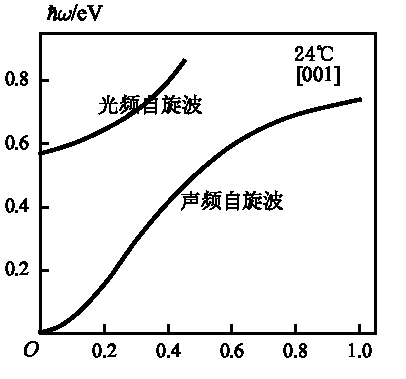
\includegraphics[width=8.5cm]{fig3-5.pdf}\\{\small 图 3.5\quad $\mathrm{Fe_3O_4}$ 中的自旋波}
\end{minipage}
\end{center}

低温比热容
\begin{equation}
  c_m=\nu Nk_{\mathrm{B}}\left(\frac{\left|S_a-S_b\right|}{4\left|J\right|S_aS_b}\right)^{3/2}
  \left(k_{\mathrm{B}}T\right)^{3/2}
\end{equation}
在计算时限于立方晶系，并且在低温区只需计算铁氧体自旋波中低频一支
$\omega_k^{(-)}$ 支的贡献，而略去 $\omega_k^{(+)}$ 支，其中的 $\alpha$ 与
$\nu$ 已在§4 中给出.
将以上结果与式(3.4.4)和式(3.4.15)相比较可见铁氧体的 $c_m$ 及 $M\left(T\right)$
也与铁磁体相似，大体上相当于
$JS\rightarrow\left|J\right|\,2S_aS_b/\left|S_a-S_b\right|$
.但是，由于铁氧体的 $J<0$
，其磁序特性又类似于反铁磁体，例如铁氧体中子格的自旋零点偏离为
\begin{equation}
  \Delta\mathcal{S}_a^{z}=\Delta\mathcal{S}_b^{z}
  =\frac{1}{2}\sum_k\left\{\left(1-c^2\gamma_k^2\right)^{-\frac{1}{2}}-1\right\}
\end{equation}
其中
\begin{equation}
  c=\frac{2\left(S_aS_b\right)^{\frac{1}{2}}}{\left(S_a+S_b\right)}
\end{equation}
当 $S_a=S_b$ 时，与反铁磁体的零点偏离公式(3.5.30)一致.

实际的铁氧体结构很复杂，例如，尖晶体型结构的铁锰氧体
$\left(\mathrm{MnFe_2O_4}\right)$ 含有 6 个 fcc
磁子晶格，应有多支自旋波谱，这将使计算变得困难.尽管如此，在长波限各支自旋波的频率与
$k^2$ 成正比的特征仍然不变.

\section{一维铁磁链中的孤波\textsuperscript{[12]}}

现在讨论磁振子之间的互作用对一维铁磁链中自旋运动的影响.设一维链中格点数为 $N$，当存在外磁场
$B$ 时一维链的各向异性海森伯模型设为
\begin{equation}
  H=-\mu B\sum_l\hat{S}_l^{z}
  -\frac{1}{2}J\sum_{l,\delta}\left(\hat{S}_l^{+}\hat{S}_{l+\delta}^{-}
  +\hat{S}_l^{-}\hat{S}_{l+\delta}^{+}\right)
  -J'\sum_{l,\delta}\hat{S}_l^{z}\hat{S}_{l+\delta}^{z}
\end{equation}
其中 $\mu\equiv g\mu_{\mathrm{B}}$，$J'>J>0$，晶格常数取为
1.为了讨论磁振子之间的相互作用，应计入非线性效应.利用近似展开式(3.3.29)，将自旋算符与场算符间的霍斯坦因－普里马可夫变换式(3.3.15)写成
\begin{equation}
  \left.\begin{aligned}
    \hat{S}_l^{z}&=S-a_l^{+}a_l\\
    \hat{S}_l^{+}&\approx\sqrt{2S}\left(1-\frac{1}{4S}a_l^{+}a_l\right)a_l\\
    \hat{S}_l^{-}&\approx\sqrt{2S}\,a_l^{+}\left(1-\frac{1}{4S}a_l^{+}a_l\right)
  \end{aligned}\right\}
\end{equation}
代入式(3.7.1)，求得准至场算符四次项的哈密顿量
\begin{equation}
\begin{aligned}
  H={}&-2J'S^2N-\mu BSN+\mu B\sum_l a_l^{+}a_l
  +S\sum_{l,\delta}\bigl\{J'\left(a_l^{+}a_l+a_{l+\delta}^{+}a_{l+\delta}\right)\\
  &-J\left(a_la_{l+\delta}^{+}+a_l^{+}a_{l+\delta}\right)\bigr\}
  -J'\sum_{l,\delta}a_l^{+}a_la_{l+\delta}^{+}a_{l+\delta}\\
  &+\frac{1}{4}J\sum_{l,\delta}\left(a_l^{+}a_{l+\delta}^{+}a_{l+\delta}a_{l+\delta}
  +a_{l+\delta}^{+}a_l^{+}a_la_l+a_l^{+}a_l^{+}a_la_{l+\delta}\right.\\
  &\qquad\qquad\left.+a_{l+\delta}^{+}a_{l+\delta}^{+}a_{l+\delta}a_l\right)
\end{aligned}
\end{equation}
算符 $a_l$ 的运动方程为
\begin{equation}
\begin{aligned}
  \mathrm{i}\hbar\frac{\partial a_l}{\partial t}&=\left(\mu B+4J'S\right)a_l
  -2JS\sum_\delta a_{l+\delta}
  -2J'\sum_\delta a_{l+\delta}^{+}a_{l+\delta}a_l\\
  &\quad+\frac{1}{2}J\sum_\delta\left(a_{l+\delta}^{+}a_{l+\delta}a_{l+\delta}
  +a_{l+\delta}^{+}a_la_l+2a_l^{+}a_la_{l+\delta}\right)
\end{aligned}
\end{equation}
这是一个非线性的算符方程.当 $B=0$
时，如果略去式(3.7.4)右边的非线性项并令 $J'=J$
，它立刻简化为式(3.3.32)，代表自旋波模式的运动方程.

上述非线性算符方程可利用相干态方法\textsuperscript{[13]}
变换为自旋运动的概率幅(probability amplitude)方程.
设系统 $H$ 的解由态 $|\Psi\rangle$ 描述，则 $l$
格点上自旋运动的概率幅可定义为
\begin{equation}
  \alpha_l\equiv\langle\Psi\mid a_l\mid\Psi\rangle
\end{equation}
$\alpha_l$
是复量，可以用 $\alpha_l$
标记各格点上自旋运动状态 $|\alpha_l\rangle$，并将系统的态用 $|\alpha_l\rangle$ 的直接乘积表示
\begin{equation}
  |\Psi\rangle=\prod_l|\alpha_l\rangle\equiv|\{\alpha_l\}\rangle
\end{equation}
根据式(3.7.5)和(3.7.6)，得到非厄密算符 $a_l$ 的本征方程
\begin{equation}
  a_l|\alpha_l\rangle=\alpha_l|\alpha_l\rangle
\end{equation}
这样确定的 $|\Psi\rangle$
称为相干态.应注意，相干态中 $|\alpha\rangle$
与§3 中确定磁振子数的状态 $|n\rangle$
不同，两者的关系可参考附录 F.
此外，在附录 F
中还证明了相干态是最小的不确定态，也可以说它是最经典的量子态，因此用相干态描述自旋的运动将是一种良好的近似.

将非线性算符方程式(3.7.4)作用于态 $|\{\alpha_l\}\rangle$
上，运用关系式(3.7.7)，容易求得概率幅方程
\begin{equation}
\begin{aligned}
  \mathrm{i}\hbar\frac{\partial\alpha_l}{\partial t}
  &=\left\{\mu B+4\left(J'-J\right)S\right\}\alpha_l
  +2JS\left(2\alpha_l-\alpha_{l+1}-\alpha_{l-1}\right)\\
  &\quad-2J'\left(\left|\alpha_{l+1}\right|^2+\left|\alpha_{l-1}\right|^2\right)\alpha_l\\
  &\quad+\frac{1}{2}J\sum_\delta\left(2\left|\alpha_l\right|^2
  +\left|\alpha_{l+\delta}\right|^2\right)\alpha_{l+\delta}
  +\frac{1}{2}J\alpha_l^2\sum_\delta\alpha_{l+\delta}^{*}
\end{aligned}
\end{equation}
当 $\alpha_l\left(t\right)$
在链中发生显著变化的空间尺度比晶格常数大得多时，可假定自旋运动的概率幅
$\alpha_l\left(t\right)$
是空间缓变量，并采用连续模型.为此，定义一个连续化的函数
$\alpha\left(x,t\right)$ 描述概率幅的时空变化
\begin{equation}
  \alpha\left(x,t\right)|_{x=l}\equiv\alpha_l\left(t\right)
\end{equation}
在连续模型近似下
\begin{equation}
  \alpha_{l\pm1}\left(t\right)-\alpha_l\left(t\right)=\pm\frac{\partial\alpha\left(x,t\right)}{\partial x}
  +\frac{1}{2}\frac{\partial^2\alpha\left(x,t\right)}{\partial x^2}+\cdots
\end{equation}
其中取晶格常数为 1.
相应的概率幅方程经上述连续化手续后，可近似写为下列非线性方程
\begin{equation}
\begin{aligned}
  \mathrm{i}\hbar\frac{\partial\alpha\left(x,t\right)}{\partial t}
  &+2JS\frac{\partial^2\alpha\left(x,t\right)}{\partial x^2}
  +4\left(J'-J\right)\left|\alpha\left(x,t\right)\right|^2\alpha\left(x,t\right)\\
  &=\left[\mu B+4\left(J'-J\right)S\right]\alpha\left(x,t\right)
\end{aligned}
\end{equation}
对上式作变换
\begin{equation*}
  \alpha\left(x,t\right)=\mathrm{e}^{-\mathrm{i}\lambda t}\phi\left(\xi,t\right)
\end{equation*}
\begin{equation}
  \xi\equiv\sqrt{\frac{\hbar}{2JS}}\,x
\end{equation}
若将参量 $\lambda$ 取为
\begin{equation}
  \hbar\lambda=\mu B+4\left(J'-J\right)S
\end{equation}
可消去式(3.7.11)右边的项，求得 $\phi\left(\xi,t\right)$ 的方程
\begin{equation*}
  \mathrm{i}\phi_t+\phi_{\xi\xi}+2Q\left|\phi\right|^2\phi=0
\end{equation*}
\begin{equation}
  Q\equiv\frac{2\left(J'-J\right)}{\hbar}>0
\end{equation}
式(3.7.14)是孤子问题中的非线性薛定谔方程(NLS)\textsuperscript{[14]}，它有标准解
\begin{equation}
  \phi\left(\xi,t\right)=A\exp\left[\mathrm{i}\,\frac{v_1}{2}\left(\xi-v_2t\right)\right]
  \mathrm{sech}\left[\sqrt{Q}\,A\left(\xi-v_2t\right)\right]
\end{equation}
其中 $A$ 为参量，$v_1$ 为积分常数，$v_2$
由上式代入非线性方程式(3.7.14)决定，当解满足方程时
\begin{equation}
  \frac{1}{2}\hbar v_1v_2=\hbar v_1^2-QA^2
\end{equation}
利用归一条件 $\int\left|\alpha\left(x,t\right)\right|^2\mathrm{d}x=1$ 可定出
$A=1/\sqrt{2L}$.相应的归一概率幅写成
\begin{equation}
  \alpha\left(x,t\right)=\frac{1}{\sqrt{2L}}
  \exp\left[\mathrm{i}\left(\gamma x-\omega t\right)\right]
  \mathrm{sech}\left[\frac{x-vt}{L}\right]
\end{equation}
其中
\begin{equation}
  L=\frac{2JS}{\left(J'-J\right)}\,,\qquad
  v=v_1\sqrt{\frac{2JS}{\hbar}}\,,\qquad
  \gamma=\frac{\hbar v}{4JS}
\end{equation}
\begin{equation}
  \hbar\omega\equiv E=\hbar\lambda+\frac{\hbar}{2}v_1v_2
  =\left[\mu B+4\left(J'-J\right)S+\frac{\hbar^2v^2}{8JS}
  -\frac{\left(J'-J\right)^2}{2JS}\right]
\end{equation}
解 $\alpha\left(x,t\right)$
代表相速为 $\left(\omega/\gamma\right)$
的振荡波，其包络是一个钟形峰，峰宽由 $L$
量度，包络中心以确定速度 $v$
在一维链中传播，传播过程中包络的形状不变，因此 $\alpha\left(x,t\right)$
振荡波的包络构成一个稳定的钟形孤波，称为包络孤子，$L$
代表包络孤子的尺寸.连续化近似要求孤子尺寸远远大于晶格常数，即必须
\begin{equation}
  L>\!>1
\end{equation}
这个条件意味着 $J'>J$，它与本节开始时的假定一致.$\hbar\omega$
代表孤波的量子.显然，它比线性自旋波理论中的磁振子能量要低
$\left(J'-J\right)^2/2JS$
量级，说明在一维铁磁链中由于非线性互作用所导致的孤波解是稳定解.当 $J'=J$ 时，
$L\rightarrow\infty$，这时由式(3.7.17)得到 $\alpha\left(x,t\right)=0$
，似乎表明对于各向同性的一维铁磁链不存在孤波解.但是实际情况并非如此，进一步的研究已经证明\textsuperscript{[15]}：如果将
$\hat{\boldsymbol{S}}_l^{\pm}$
的变换式(3.3.15)展开到更高阶项（包括 $S^0,S^{-1},S^{-2}$
项），即使是各向同性情况也可求得包络孤子解.

因此，我们可以说一维铁磁链中包络孤子解的存在是磁振子之间互作用所导致的.除包络孤子外，在一维磁体中还存在其它类型的孤子解，如扭型孤子解和脉冲状孤子解等.目前磁性孤子已经证实是低维系中自旋运动的一种模式，它代表系统的非线性元激发，20
世纪 80
年代以来在理论和实验研究方面都有较大进展\textsuperscript{[16]}.

\begin{canKao}
\begin{enumerate}[label={[\arabic*]}, leftmargin=2.2em, itemsep=0pt]
\item Heisenberg W. Phys Z, 1928, 49: 619
\item Dirac PAM. Proc Roy Soc, 1929, A123: 714
\item Anderson PW. Solid State Phys, 1963, 14: 99
\item Kittel C. Quantum Theory of Solids. New York: John Wiley \& Sond, Inc, 1963
\item Holstein T, Primakoff H. Phys Rev, 1940, 58: 1098
\item Dietrich OW {\it et al}. Phys Rev, 1976, B14: 4932
\item Bloch F. Z. Phys, 1930, 61: 206
\item Dyson F J. Phys Rev, 1956, 102: 1217, 1230
\item Bogoliubov N N. J Phys USSR, 1947, 11: 23
\item Anderson P W. Phys Rev, 1952, 86: 694
\item Jacobs LS. J. Appl Phys, 1961, 32: 615
\item Pushkarov D I {\it et al}. Phys Lett, 1977, 61A: 339
\item Glauber R J. Phys Rev, 1963, 131: 2766
\item Eilenberger G. Solitons. Berlin: Spinger-Verlag, 1981
\item Cordeiro C E {\it et al}. Phys Lett, 1978, 66A: 332
\item 蒲富恪，李伯臧.一维磁体中磁性孤子研究的进展.第五届全国磁学会议.1983
\end{enumerate}
\end{canKao}
